\documentclass[a4paper,12pt,twoside]{memoir}

% Castellano
\usepackage[spanish,es-tabla]{babel}
\selectlanguage{spanish}
\usepackage[utf8]{inputenc}
\usepackage[T1]{fontenc}
\usepackage{lmodern} % scalable font
\usepackage{microtype}
\usepackage{placeins}

\RequirePackage{booktabs}
\RequirePackage[table]{xcolor}
\RequirePackage{xtab}
\RequirePackage{multirow}

% Links
\PassOptionsToPackage{hyphens}{url}\usepackage[colorlinks]{hyperref}
\hypersetup{
	allcolors = {red}
}

% Ecuaciones
\usepackage{amsmath}

% Rutas de fichero / paquete
\newcommand{\ruta}[1]{{\sffamily #1}}

% Párrafos
\nonzeroparskip

% Huérfanas y viudas
\widowpenalty100000
\clubpenalty100000

% Evitar solapes en el header
\nouppercaseheads

% Imagenes
\usepackage{graphicx}
\newcommand{\imagen}[2]{
	\begin{figure}[!h]
		\centering
		\includegraphics[width=0.9\textwidth]{#1}
		\caption{#2}\label{fig:#1}
	\end{figure}
	\FloatBarrier
}

\newcommand{\imagenflotante}[2]{
	\begin{figure}%[!h]
		\centering
		\includegraphics[width=0.9\textwidth]{#1}
		\caption{#2}\label{fig:#1}
	\end{figure}
}



% El comando \figura nos permite insertar figuras comodamente, y utilizando
% siempre el mismo formato. Los parametros son:
% 1 -> Porcentaje del ancho de página que ocupará la figura (de 0 a 1)
% 2 --> Fichero de la imagen
% 3 --> Texto a pie de imagen
% 4 --> Etiqueta (label) para referencias
% 5 --> Opciones que queramos pasarle al \includegraphics
% 6 --> Opciones de posicionamiento a pasarle a \begin{figure}
\newcommand{\figuraConPosicion}[6]{%
  \setlength{\anchoFloat}{#1\textwidth}%
  \addtolength{\anchoFloat}{-4\fboxsep}%
  \setlength{\anchoFigura}{\anchoFloat}%
  \begin{figure}[#6]
    \begin{center}%
      \Ovalbox{%
        \begin{minipage}{\anchoFloat}%
          \begin{center}%
            \includegraphics[width=\anchoFigura,#5]{#2}%
            \caption{#3}%
            \label{#4}%
          \end{center}%
        \end{minipage}
      }%
    \end{center}%
  \end{figure}%
}

%
% Comando para incluir imágenes en formato apaisado (sin marco).
\newcommand{\figuraApaisadaSinMarco}[5]{%
  \begin{figure}%
    \begin{center}%
    \includegraphics[angle=90,height=#1\textheight,#5]{#2}%
    \caption{#3}%
    \label{#4}%
    \end{center}%
  \end{figure}%
}
% Para las tablas
\newcommand{\otoprule}{\midrule [\heavyrulewidth]}
%
% Nuevo comando para tablas pequeñas (menos de una página).
\newcommand{\tablaSmall}[5]{%
 \begin{table}
  \begin{center}
   \rowcolors {2}{gray!35}{}
   \begin{tabular}{#2}
    \toprule
    #4
    \otoprule
    #5
    \bottomrule
   \end{tabular}
   \caption{#1}
   \label{tabla:#3}
  \end{center}
 \end{table}
}

%
%Para el float H de tablaSmallSinColores
\usepackage{float}

%
% Nuevo comando para tablas pequeñas (menos de una página).
\newcommand{\tablaSmallSinColores}[5]{%
 \begin{table}[H]
  \begin{center}
   \begin{tabular}{#2}
    \toprule
    #4
    \otoprule
    #5
    \bottomrule
   \end{tabular}
   \caption{#1}
   \label{tabla:#3}
  \end{center}
 \end{table}
}

\newcommand{\tablaApaisadaSmall}[5]{%
\begin{landscape}
  \begin{table}
   \begin{center}
    \rowcolors {2}{gray!35}{}
    \begin{tabular}{#2}
     \toprule
     #4
     \otoprule
     #5
     \bottomrule
    \end{tabular}
    \caption{#1}
    \label{tabla:#3}
   \end{center}
  \end{table}
\end{landscape}
}

%
% Nuevo comando para tablas grandes con cabecera y filas alternas coloreadas en gris.
\newcommand{\tabla}[6]{%
  \begin{center}
    \tablefirsthead{
      \toprule
      #5
      \otoprule
    }
    \tablehead{
      \multicolumn{#3}{l}{\small\sl continúa desde la página anterior}\\
      \toprule
      #5
      \otoprule
    }
    \tabletail{
      \hline
      \multicolumn{#3}{r}{\small\sl continúa en la página siguiente}\\
    }
    \tablelasttail{
      \hline
    }
    \bottomcaption{#1}
    \rowcolors {2}{gray!35}{}
    \begin{xtabular}{#2}
      #6
      \bottomrule
    \end{xtabular}
    \label{tabla:#4}
  \end{center}
}

%
% Nuevo comando para tablas grandes con cabecera.
\newcommand{\tablaSinColores}[6]{%
  \begin{center}
    \tablefirsthead{
      \toprule
      #5
      \otoprule
    }
    \tablehead{
      \multicolumn{#3}{l}{\small\sl continúa desde la página anterior}\\
      \toprule
      #5
      \otoprule
    }
    \tabletail{
      \hline
      \multicolumn{#3}{r}{\small\sl continúa en la página siguiente}\\
    }
    \tablelasttail{
      \hline
    }
    \bottomcaption{#1}
    \begin{xtabular}{#2}
      #6
      \bottomrule
    \end{xtabular}
    \label{tabla:#4}
  \end{center}
}

%
% Nuevo comando para tablas grandes sin cabecera.
\newcommand{\tablaSinCabecera}[5]{%
  \begin{center}
    \tablefirsthead{
      \toprule
    }
    \tablehead{
      \multicolumn{#3}{l}{\small\sl continúa desde la página anterior}\\
      \hline
    }
    \tabletail{
      \hline
      \multicolumn{#3}{r}{\small\sl continúa en la página siguiente}\\
    }
    \tablelasttail{
      \hline
    }
    \bottomcaption{#1}
  \begin{xtabular}{#2}
    #5
   \bottomrule
  \end{xtabular}
  \label{tabla:#4}
  \end{center}
}



\definecolor{cgoLight}{HTML}{EEEEEE}
\definecolor{cgoExtralight}{HTML}{FFFFFF}

%
% Nuevo comando para tablas grandes sin cabecera.
\newcommand{\tablaSinCabeceraConBandas}[5]{%
  \begin{center}
    \tablefirsthead{
      \toprule
    }
    \tablehead{
      \multicolumn{#3}{l}{\small\sl continúa desde la página anterior}\\
      \hline
    }
    \tabletail{
      \hline
      \multicolumn{#3}{r}{\small\sl continúa en la página siguiente}\\
    }
    \tablelasttail{
      \hline
    }
    \bottomcaption{#1}
    \rowcolors[]{1}{cgoExtralight}{cgoLight}

  \begin{xtabular}{#2}
    #5
   \bottomrule
  \end{xtabular}
  \label{tabla:#4}
  \end{center}
}




\graphicspath{ {./img/} }

% Capítulos
\chapterstyle{bianchi}
\newcommand{\capitulo}[2]{
	\setcounter{chapter}{#1}
	\setcounter{section}{0}
	\setcounter{figure}{0}
	\setcounter{table}{0}
	\chapter*{#2}
	\addcontentsline{toc}{chapter}{#2}
	\markboth{#2}{#2}
}

% Apéndices
\renewcommand{\appendixname}{Apéndice}
\renewcommand*\cftappendixname{\appendixname}

\newcommand{\apendice}[1]{
	%\renewcommand{\thechapter}{A}
	\chapter{#1}
}

\renewcommand*\cftappendixname{\appendixname\ }

% Formato de portada
\makeatletter
\usepackage{xcolor}
\newcommand{\tutor}[1]{\def\@tutor{#1}}
\newcommand{\course}[1]{\def\@course{#1}}
\definecolor{cpardoBox}{HTML}{E6E6FF}
\def\maketitle{
  \null
  \thispagestyle{empty}
  % Cabecera ----------------
\noindent
\includegraphics[width=\textwidth]{cabecera}\vspace{1cm}%
  \vfill
  % Título proyecto y escudo informática ----------------
  \colorbox{cpardoBox}{%
    \begin{minipage}{.8\textwidth}
      \vspace{.5cm}\Large
      \begin{center}
      \textbf{TFG del Grado en Ingeniería Informática}\vspace{.6cm}\\
      \textbf{\LARGE\@title{ }}
      \end{center}
      \vspace{.2cm}
    \end{minipage}

  }%
  \hfill\begin{minipage}{.20\textwidth}
    
\includegraphics[width=\textwidth]{escudoInfor}
  \end{minipage}
  \vfill
  % Datos de alumno, curso y tutores ------------------
  \begin{center}%
  {%
    \noindent\LARGE
    Presentado por \@author{}\\ 
    en Universidad de Burgos --- \@date{}\\
    Tutor: \@tutor{}\\
  }%
  \end{center}%
  \null
  \cleardoublepage
  }
\makeatother


% Datos de portada
\title{Estudio y configuración de un sistema ELK  \\Documentación Técnica}
\author{Hugo de la Cámara Saiz}
\tutor{Jesús Manuel Maudes Raedo }
\date{\today}

\begin{document}

\maketitle



\cleardoublepage



%%%%%%%%%%%%%%%%%%%%%%%%%%%%%%%%%%%%%%%%%%%%%%%%%%%%%%%%%%%%%%%%%%%%%%%%%%%%%%%%%%%%%%%%



\frontmatter


\clearpage

% Indices
\tableofcontents

\clearpage

\listoffigures

\clearpage

\listoftables

\clearpage

\mainmatter

\appendix

\apendice{Plan de Proyecto Software}

\section{Introducción}
En este apartado de la documentación de los anexos se pretende exponer de manera cronológica como ha ido evolucionando el desarrollo del estudio realizado.

Durante la maduración del mismo se ha empleado la metodología \textit{Scrum} para dividir cada fase del proyecto en \textit{sprints}, dentro de cada cuál se incluye una planificación, un desarrollo y una revisión en forma de reunión del mismo.

A lo largo del desarrollo del estudio, se han ido anotando todas las tareas solicitadas para cada sprint en el \href{https://github.com/hds1001/Estudio-y-configuracion-de-un-sistema-ELK}{repositorio} GitHub del proyecto, por lo que en este apartado se hará un desglose de cada tarea involucrada.

Además de todo lo mencionado anteriormente, también se va a estudiar la viabilidad del proyecto, tanto económica, como legal.

\paragraph{}
\paragraph{}
\paragraph{}
\paragraph{}
\paragraph{}


\section{Planificación temporal}

\subsection{Sprint 1 (15/02 - 17/03)}
\subsubsection{Planificación}
Tras una primera toma de contacto entre los miembros del estudio, se acordó que inicialmente se comenzaría con un trabajo de investigación sobre el funcionamiento de cada componente de un sistema basado en ELK, así como la instalación de los mismos y prueba de que se ejecutaban correctamente.

También se encomendó la tarea de crear el repositorio GitHub del estudio, en el que se irían actualizando, a medida que se avanzaba las \textit{issues} del proyecto.

\subsubsection{Issues}
\begin{itemize}
    \item \textbf{Investigación e instalación de Kibana}
    \item \textbf{Investigación e instalación de ElasticSearch}
    \item \textbf{Investigación e instalación de Logstash}
    \item \textbf{Configuración del repositorio GitHub}
    \item \textbf{Inicio documentación de la memoria}

    \end{itemize}

\subsubsection{Desarrollo}
En este primer mes se investigó a través de las fuentes principales de información de cada programa su instalación y uso básico de cara a probar con pruebas lo que ofrecían. En primer lugar ElasticSearch no opuso grandes dificultades, puesto que posee una extensa documentación, y su ejecución fue relativamente sencilla, cosa que no ocurrió con Logstash, ya que su comprensión era más compleja y requería de conocimientos más elevados que para las otros dos componentes. Por último, en Kibana fue en el que más profundizo en este sprint, puesto que era el programa más intuitivo que más posibilidades y complementos ofrecía.

También se hizo énfasis en analizar programas alternativos a estos comparando las ventajas e inconvenientes frente a Elastic, Logstash y Kibana.

\subsubsection{Revisión}
En la segunda reunión se compartieron los resultados encontrados y por parte del tutor el programa que más interés desperto fue Logstash, puesto que las opciones que ofrecía erán las más interesantes de estudiar, cimentando así las bases del segundo sprint que comenzaría inmediatamente después.

\subsection{Sprint 2 (18/03 - 03/04)}
\subsubsection{Planificación}
En esta segunda fase del proyecto, una vez conocidas las características básicas de los componentes y como se relacionan entre sí, se creyó conveniente profundizar en las posibilidades de filtrado que ofrece Logstash, sabiendo diferenciar qué se puede y qué no se puede hacer.

También se empezó a mencionar la idea de aplicar tanto Machine Learning como MapReduce en algún momento del proceso a los datos, por lo que se encomendó el comienzo de la investigación de ambos temas.

\subsubsection{Issues}
\begin{itemize}
    \item \textbf{Comenzar con la documentación de la memoria en LaTeX}
    \item \textbf{Investigar sobre la funcionalidad de Machine Learning en Elastic}
    \item \textbf{Investigar funcionamiento filtrado Logstash}
    \item \textbf{Investigar desarrollo con plugins en ElasticSearch}
    \item \textbf{Investigar posible integración con Python para el tratamiento de datos}
    \item \textbf{Investigar desarrollo con Docker y como integrarlo}
    \item \textbf{Investigar funcionamiento MapReduce en Logstash}
    \item \textbf{Investigar funcionamiento MapReduce en ElasticSearch}
    \item \textbf{Investigar funcionamiento MapReduce en Kibana}
    \item \textbf{Probar filtrado en Logstash: sumas, agrupamientos, discretizar columna numérica}
    \item \textbf{Continuar con documentación en Overleaf}
    \item \textbf{Familiarización con librería SKLearn en cuanto a clasificación, regresión, clustering y PCA}
\end{itemize}

\subsubsection{Desarrollo}
Se investigó la posibilidad que ofrecía el plugin de Machine Learning que ofrece ElasticSearch, cuyas funciones gratuitas son limitadas, y las más interesantes son de pago. Por parte del tutor, se ofreció una fuente de información para poder aplicar funciones de Machine Learning de manera gratuita a fuentes de datos, \textit{Scikit-Learn}, de manera que durante este tiempo el estudio se enfocó en comprender el funcionamiento de esta librería, y de qué manera la podíamos acoplar en el sistema ELK.

Por otro lado, indagar en las funciones avanzadas de Logstash, fue costoso, puesto que la información presente en internet era escasa y la mayoría antigua, por lo que las pruebas con este programa fueron un claro ensayo y error hasta dar con la tecla. Se profundizo en las operaciones de filtrado, agrupamientos básicos y discretizaciones en el apartado \textit{filter} de el archivo de configuración.

\subsubsection{Revisión}
En la tercera y cuarta reunión entre los miembros se discutió sobre qué filtros erán más interesantes de aplicar, el orden que debían seguir los datos a lo largo de todo el proceso ETL, y cómo se podían integrar los resultados obtenidos por las funciones de \textit{Scikit-Learn} en Elastic para su posterior exposición en Kibana. Concluyendo así el segundo sprint del proyecto y abriendo temas para la tercera fase.

\paragraph{}
\paragraph{}
\paragraph{}
\paragraph{}
\paragraph{}

\subsection{Sprint 3 (04/04  - 20/04)}
\subsubsection{Planificación}
Y así entramos en la tercera etapa del estudio, en la que se plantearon tareas a realizar como la carga con éxito de los datos del script del Iris en Kibana, continuar explorando los filtros de Logstash, y abordar el tema los \textit{streamings} de datos, que aún no estaba desarrollado en este momento del estudio.

Otro punto a destacar como importante de cara a realizar en esta fase, es el de conseguir realizar de manera eficiente y útil  MapReduce en Logstash.

\subsubsection{Issues}
\begin{itemize}
    \item \textbf{Cargar datos Iris en Kibana}
    \item \textbf{Explorar más posibilidades de agrupamiento en Logstash con máximos, medias, etc.}
    \item \textbf{Probar Data Streams: los que se puede y no (funcionamiento, campos, etc.)} 
    \item \textbf{Comparar MapReduce en Kibana con Logstash}
    \item \textbf{Probar Data Streams: los que se puede y no (funcionamiento, campos, etc.)}
\end{itemize}

\subsubsection{Desarrollo}
Por un lado, gracias a los foros presentes en las páginas oficiales tanto de Elastic como de \textit{Scikit-Learn}, se consiguió combinar los dos, de manera que el tráfico de información entre ambos fuera fluido y exitoso. Esto se hizo tras realizarle unas modificaciones al script tanto en la forma en la que ingestaba los datos, como en la de como se exportaban los mismos, y hacia donde.

El tema de los \textit{data streams} siguió sin avanzar, puesto que no se encontraba de qué manera se podía implementar esta forma de ingesta de datos en el sistema ELK. 

Y trás darle unas cuantas vueltas, se llegó a la conclusión de que la manera de realizar el MapReduce en Logstash era con su función \textit{aggregate}.

\subsubsection{Revisión}
Así se cubrió lo relacionado con \textit{Scikit-Learn} de manera parcial y cubriendo la tarea encomendada, mientras que los \textit{streamings} de datos en vivo seguía en el aire y sin saber muy bien hacia donde seguir tirando.

\subsection{Sprint 4 (22/04 - 30/04)}
\subsubsection{Planificación}
Para este cuarto sprint, se vió que el tema de los \textit{data streams} había que terminarlo, por lo que se le dió máxima relevancia a este, de manera que se pudieran mandar datos en tiempo real a Elastic de manera que se les aplicara un filtrado con Logstash y pudieran ser expuestos en Kibana.

\subsubsection{Issues}
\begin{itemize}
        \item \textbf{Probar funcionamiento Data Streams}   
    \item \textbf{Investigar funcionamiento WebSocket en ELK}
        \item \textbf{Conectar WebSocket con Logstash}
\end{itemize}

\subsubsection{Desarrollo}
Esto se logró gracias a las herramientas \textit{WebSocket}, la cuál permitio poder conectarnos a una fuente de datos, \textit{Finnhub}, que mandara los datos tanto a Elastic como a Logstash, y esos datos fueran depurados para ser mostrados en un \textit{dashboard} de Kibana. Esto se consiguió gracias a un \href{https://github.com/ColinEberhardt/awesome-public-streaming-datasets}{repositorio} público de GitHub que ofrecía diferentes maneras de interactuar con datos en vivo.

De manera paralela a los \textit{WebSockets}, se trabajó con una herramienta del ecosistemas Elastic llamada \textit{Filebeat}, la cuál ofrecía cubir la necesidad de poder mandar datos en \textit{streaming} hacia Elastic o Logstash, pero al ver que la alternativa encontrada era más eficiente y ofrecía más posibilidades, se optó por los \textit{WebSockets}.

\subsubsection{Revisión}
En la sexta reunión de los miembros se mostró tranquilidad al ver que gran parte de los problemas presentes habían sido solventados y que se comprendía de que manera se podían implementar \textit{data streams} en el sistema ELK.

Con esto, se empezó a plantear la posibilidad de empezar a preparar los escenarios finales junto con la documentación de el funcionamiento de cada uno.

\subsection{Sprint 5 (31/04 - 06/05)}
\subsubsection{Planificación}
Por lo que en la séptima reunión se hizo retrospectiva de lo que se tenía hasta el momento, y se decidió que el tema de las transformaciones de datos en Logstash aún no estaba en un buen punto, por lo que en este sprint se centró el tiempo en cerrar todo esto.

También se dió enfásis a la idea del \textit{Edge Computing}, y como podía ser relevante aplicarlo en el estudio.

\subsubsection{Issues}
\begin{itemize} 
    \item \textbf{Estudiar posibilidad hacer MapReduce del data stream en Logstash}  
    \item \textbf{Investigar funcionamiento MapReduce en Kibana}    
    \item \textbf{Investigar sobre el Edge Computing y como funciona} 
\end{itemize}

\subsubsection{Desarrollo}
Finalmente se terminó de cerrar todo lo relacionado con los filtrados en Logstash al aplicar distintas funciones a una fuente de datos. Funciones como:
\begin{itemize}
    \item Borrar campos vacíos
    \item Transformación de tipos
    \item Operaciones con distintos campos
\end{itemize}

Por otra parte, hubo un trabajo de investigación sobre \textit{Edge Computing} de cara a poder documentarlo en la memoria, y se comprendió la idea que se le asociaba.

\subsubsection{Revisión}
Así se concluyó esta quinta fase, dando por sentados todos los escenarios que iban a estar presentes en la documentación técnica, y se comenzó a plantear la idea de la preparación e ilustración de los mismos.

\subsection{Sprint 6 (07/05 - 16/05)}
\subsubsection{Planificación}
Llegando a esta sexta etapa ya se empezaba a divisar el final en el horizonte y se encomendó la tarea de ilustrar y preparar minuciosamente cada escenario tratado de manera que la documentación de los mismos fuera más sencilla.

\subsubsection{Issues}
\begin{itemize}
    \item \textbf{Estudiar caso importar directamente el fichero en Elastic}
    \item \textbf{Estudiar caso importar el fichero desde Logstash}
    \item \textbf{Estudiar caso importar un DataSet (Iris)}
    \item \textbf{Estudiar caso importar a través de WebSocket a Elastic}
    \item \textbf{Estudiar caso importar a través de un WebSocket con Logstash}

    \end{itemize}
    

\subsubsection{Desarrollo}
Durante este tiempo se trabajó en preparar todos los directorios con la información relevante de cada escenario, así como ilustrar los \textit{dashboards} finales obtenidos en cada uno.

Se empezó a documentar en \textit{Overleaf}  la memoria del estudio de manera básica para ir teniendo un punto de partida.

\subsubsection{Revisión}
Tras la novena reunión de miembros se empezaron a realizar correcciones a la memoria y reestructuraciones a los escenarios de manera que las ideas presentadas fueran más claras y concisas.

\subsection{Sprint 7 (17/05 - 10/06)}
\subsubsection{Planificación}
En esta séptima etapa se continuó con el plan pensado para la anterior de seguir documentando los escenarios y los diferentes apartados de la memoria técina del estudio.

\subsubsection{Issues}
\begin{itemize}


    \item \textbf{Investigar sobre el caso de Edge Computing y cómo funciona}
    \item \textbf{Continuar desarrollo de escenarios}



\end{itemize}

\subsubsection{Desarrollo}
Por lo que todo este tiempo se dedicó a realizar modificaciones y continuar agregando información a la memoria corrigiendo la estructura y los contenidos de cada apartado de manera que fuerán más acordes a un trabajo científico.

\subsubsection{Revisión}
Siguiendo la pauta de la anterior reunión las reuniones octava y novena estuvieron enfocadas a seguir mejorando el trabajo realizado en al documentación.

\subsection{Sprint 8 (11/06 - 10/07)}
\subsubsection{Planificación}
Tras una serie de revisiones tanto de la documentación de los anexos como de la memoria, se han planteado diversas mejoras en ambos por parte del tutor. También se ha mencionado el modificar el script en el que se aplica Machine Learning, de manera que los datos se carguen desde Elastic y una vez procesados sean devueltos. Para terminar se encomendó la tarea de realizar videos explicativos del proyecto, el pulido final del repositorio y la creación de una máquina virtual que contenga todo lo relacionado con el proyecto.

\subsubsection{Issues}
\begin{itemize}


    \item \textbf{Documentación de la memoria}
    \item \textbf{Documentación de los anexos}



\end{itemize}

\subsubsection{Desarrollo}
Se dedicó todo el último mes a pulir detalles en la documentación de manera satisfactoria mediante una serie de revisiones. Se consiguió modificar la fuente de ingesta del script de Machine Learning con éxito, y se trabajó en todo lo mencionado para que la entrega del proyecto se pudiera hacer en fecha.

\subsubsection{Revisión}
Tras una última revisión de los contenidos, ambas partes quedaron satisfechas con el resultado y se acordó que esa era el producto final a entregar.

\paragraph{}
\paragraph{}
\paragraph{}
\paragraph{}
\paragraph{}
\paragraph{}
\paragraph{}
\paragraph{}
\paragraph{}
\paragraph{}
\paragraph{}
\paragraph{}

\section{Estudio de viabilidad}

\subsection{Viabilidad económica}
A lo largo de este estudio se ha empleado una versión gratuita de Elastic, en la cual, por ejemplo, el plugin que habilita la función Machine Learning, está bloqueado. Elastic ofrece esta y más funciones en sus diferentes niveles de suscripción:

\begin{enumerate}
    \item \textbf{Basic (Gratis)}
\begin{itemize}
        \item Ofrece un amplio mercado de plugins y de características limitadas, entre las cuales no se encuentra la de aplicar Machine Learning a los índices de datos. Se ofrecen integraciones para transmitir logs, métricas, rastreos, contenido y más desde diferentes fuentes. 
    \end{itemize}
    \item \textbf{Gold (109 doláres al mes)}
    \begin{itemize}
        \item Ofrece características adicionales de seguridad, monitoreo de datos y algunas funciones de Machine Learning.
    \end{itemize}
    \item \textbf{Platinum (125 doláres al mes)}
    \begin{itemize}
        \item Ofrece todas las características del nivel Gold, además de acceso completo a las capacidades de Machine Learning, alertas avanzadas, y soporte premium.
    \end{itemize}
    \item \textbf{Enterprise (175 dólares al mes)}
    \begin{itemize}
        \item Ofrece todas las características del nivel Platinum, con funcionalidades adicionales de administración de los datos y un mejor soporte.
    \end{itemize}
\end{enumerate}

Sklearn no supone coste alguno puesto que es una herramienta de código abierto. El \textit{hardware} empleado ha sido un ordenador de unos 500€.

Suponiendo que en este trabajo se han invertido unas 600 horas de trabajo a lo largo de 5 meses, que son aproximadamente 21 semanas. Asignando unas 28 horas de carga de trabajo semanal, y teniendo en cuenta que el salario del alumno será de 18€/hora, se obtiene un salario bruto de entorno a 2000€/mes. Este salario una vez se le aplica las deducciones por impuestos indicadas en la \href{https://www.seg-social.es/wps/portal/wss/internet/Trabajadores/CotizacionRecaudacionTrabajadores/36537}{página de la seguridad social} (ver figuras \ref{fig:coti1} y \ref{fig:coti2}).

\begin{figure}
    \centering
    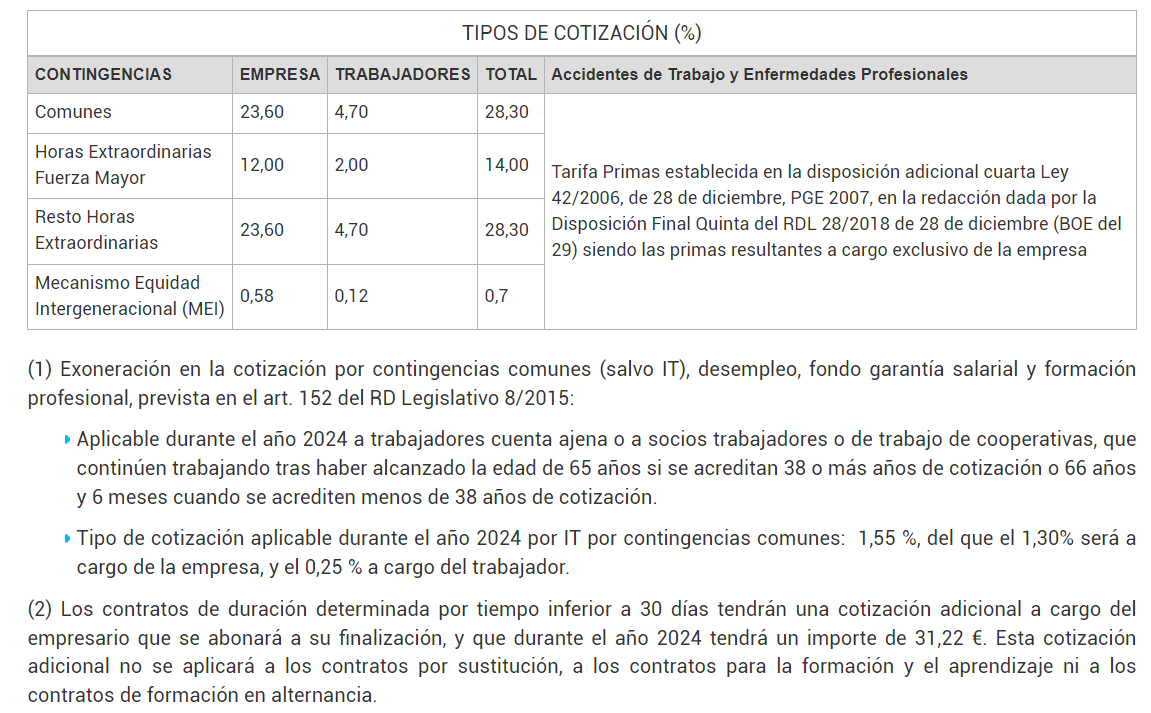
\includegraphics[width=1\linewidth]{img/cotizacion1.png}
    \caption{Tipos de cotización en el régimen general de la Seguridad Social.}
    \label{fig:coti1}
\end{figure}

\begin{figure}
    \centering
    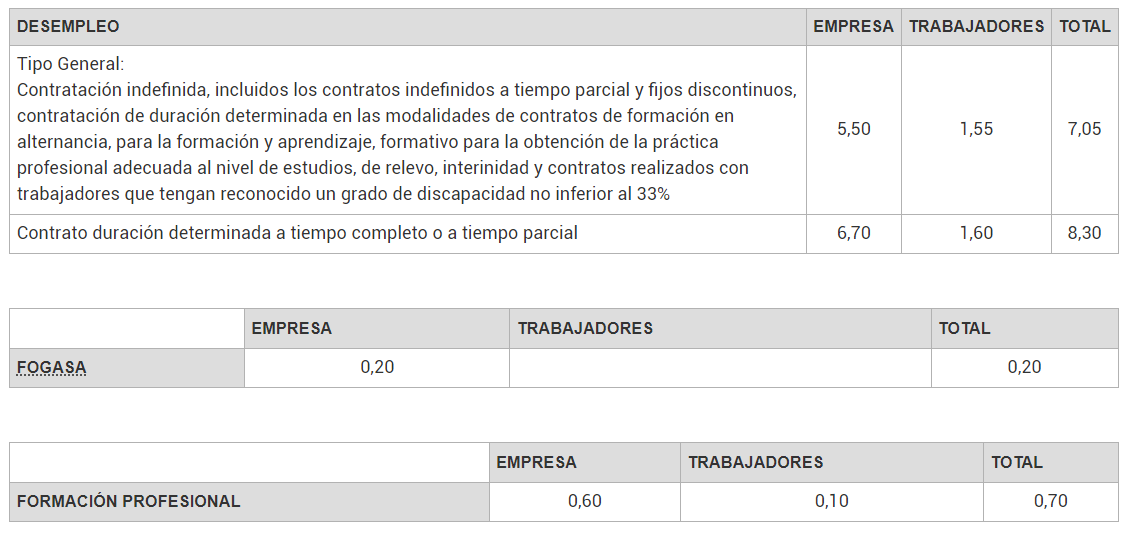
\includegraphics[width=1\linewidth]{img/cotizacion2.png}
    \caption{Más tipos de cotización en el régimen general de la Seguridad Social.}
    \label{fig:coti2}
\end{figure}

Los impuestos supondrán un 23,6 por ciento del sueldo en concepto de contingencias, un 5,5 por ciento en concepto de desempleo, un 0,2 en concepto de FOGASA y un 0,6 en concepto de formación profesional por parte de la empresa. Aplicando todos estos porcentajes el sueldo real del alumno alcanzaría la cifra de 2853€/mes.

Además del alumno también hay que tener en cuenta que se trabaja con dos profesores cumpliendo el rol de tutores. Siendo el salario mensual de 38€, y suponiendo que que trabajan 2 horas por semana, el sueldo bruto de los dos profesores será de 608€/mes, que con la aplicación de impuestos se queda en 867€/mes reales.

Una vez se tienen los datos sobre la mesa, el gasto mensual que supone el proyecto en total es de 3461€, que multiplicado por los 5 meses de duración del trabajo se quedan en 17305€ de coste total.

\subsection{Viabilidad legal}
Un sistema ELK usa principalmente dos tipos de licencias: 
\begin{itemize}
    \item La Licencia de Apache 2.0 para versiones anteriores a la 7.11. Esta licencia permite un uso comercial, de distribución, modificación y patente incluyendo un aviso de \textit{copyright} y de licencia.
    \item La Licencia Elastic para versiones a partir de la 7.11. Esta también ofrece licencias básicas gratuitas y comerciales para acceso a funciones avanzadas y soporte técnico.
    \item Sklearn posee una licencia BSD 3-Clause que otorga permisos comerciales, de distribución y modificación incluyendo un aviso de \textit{copyright} y de licencia.
\end{itemize}


\apendice{Especificación de Requisitos}

\section{Introducción}

Este apéndice ha sido modificado de una escpecificación de requisitos convencial, en lugar de exponer los diferentes requisitos, estos van a ser sustituidos por los escenarios analizados en el proyecto, adaptando así este anexo a la forma del estudio.


\section{Objetivos generales}
El objetivo de este estudio ha sido el de hacer un estudio de diferentes escenarios modificando la fuente de ingesta de un sistema ELK. En este anexo se van a hacer un desglose de cada uno de esos escenarios.

\section{Catálogo de requisitos}
\begin{enumerate}
    \item \textbf{Escenario 1: ingesta de fichero desde Elastic }
    \item \textbf{Escenario 2: ingesta de fichero desde Logstash }
    \item \textbf{Escenario 3: ingesta desde WebSocket a Elastic }
    \item \textbf{Escenario 4: ingesta de WebSocket desde Logstash }
    \item \textbf{Escenario 5: ingesta de data stream desde Logstash aplicando MapReduce }
    \item \textbf{Escenario de aplicación de Machine Learning a un conjunto de datos}
\end{enumerate}


\section{Especificación de requisitos}

Para adaptar este apartado al estudio, en esta sección se va a exponer cada escenario realizado como si fuera un caso de uso, adaptando la plantilla de manera que se adecue a la información que se quiere mostrar
\begin{table}[p]
	\centering
	\begin{tabularx}{\linewidth}{ p{0.21\columnwidth} p{0.71\columnwidth} }
		\toprule
		\textbf{CU-1}    & \textbf{Escenario 1: ingesta de fichero desde Elastic}\\
		\toprule
		\textbf{Versión}              & 1.0    \\
		\textbf{Autor}                & Hugo de la Cámara Saiz \\
		\textbf{Descripción}          & En este escenario se pretende ingestar un fichero de tipo CSV directamente desde Elastic sin intermediarios. \\
		\textbf{Precondición}         & Tener un fichero con datos en formato CSV en el sistema local  \\
		\textbf{Acciones}             &
		\begin{enumerate}
			\def\labelenumi{\arabic{enumi}.}
			\tightlist
			\item Importar el archivo desde el menú de Elastic
                \item Mostrar en un dashboard visualizaciones de los datos.
		\end{enumerate}\\
            \textbf{Postcondiciones}             &
		\begin{enumerate}
			\def\labelenumi{\arabic{enumi}.}
			\tightlist
			\item Comprobar en el Index Management que el índice se ha generado correctamente
			\item Comprobar en el Discoverer que el contenido del archivo ha sido importado correctamente.
		\end{enumerate}\\
		\textbf{Importancia}          & Alta \\
		\bottomrule
	\end{tabularx}
	\caption{CU-1 Escenario 1: ingesta de fichero desde Elastic}
\end{table}

\begin{table}[p]
	\centering
	\begin{tabularx}{\linewidth}{ p{0.21\columnwidth} p{0.71\columnwidth} }
		\toprule
		\textbf{CU-2}    & \textbf{Escenario 2: ingesta de fichero desde Logstash}\\
		\toprule
		\textbf{Versión}              & 1.0    \\
		\textbf{Autor}                & Hugo de la Cámara Saiz \\
		\textbf{Descripción}          & En este escenario se pretende ingestar un fichero de tipo log desde Logstash aplicándole una serie de transformaciones y mandarlo a Elastic posteriormente. \\
		\textbf{Precondición}         & Tener el fichero .log en el sistema local \\
		\textbf{Acciones}             &
		\begin{enumerate}
			\def\labelenumi{\arabic{enumi}.}
			\tightlist
			\item Crear un archivo .conf para Logstash en el que se le indique la ruta al input de los datos.
                \item Modificar en la sección filter las diferentes transformaciones que se quieren aplicar.
                \item Indicar en la sección output que se quiere mandar a ElasticSearch los datos procesados.
                \item Ejecutar Logstash con el archivo de configuración creado.
                \item Mostrar en un dashboard visualizaciones de los datos.
		\end{enumerate}\\
            \textbf{Postcondiciones}             &
		\begin{enumerate}
			\def\labelenumi{\arabic{enumi}.}
			\tightlist
			\item Comprobar en el Index Management que el índice se ha generado correctamente
			\item Comprobar en el Discoverer que el contenido del archivo ha sido importado correctamente.
		\end{enumerate}\\
		\textbf{Importancia}          & Alta \\
		\bottomrule
	\end{tabularx}
	\caption{CU-2 Escenario 2: ingesta de fichero desde Logstash}
\end{table}

\begin{table}[p]
	\centering
	\begin{tabularx}{\linewidth}{ p{0.21\columnwidth} p{0.71\columnwidth} }
		\toprule
		\textbf{CU-3}    & \textbf{Escenario 3: ingesta desde WebSocket a Elastic}\\
		\toprule
		\textbf{Versión}              & 1.0    \\
		\textbf{Autor}                & Hugo de la Cámara Saiz \\
		\textbf{Descripción}          & En este escenario se pretende ingestar un data stream desde un WebSocket directamente a Elastic, sin intermediarios. \\
		\textbf{Precondición}         & Disponer de una fuente de datos websocket  \\
		\textbf{Acciones}             &
		\begin{enumerate}
			\def\labelenumi{\arabic{enumi}.}
			\tightlist
			\item Configurar la fuente de datos websocket para insgestar los datos directamente en ElasticSearch.
                \item Mostrar en un dashboard visualizaciones de los datos.
		\end{enumerate}\\
             \textbf{Postcondiciones}             &
		\begin{enumerate}
			\def\labelenumi{\arabic{enumi}.}
			\tightlist
			\item Comprobar en el Index Management que el índice se ha generado correctamente
			\item Comprobar en el Discoverer que el contenido del archivo ha sido importado correctamente.
		\end{enumerate}\\
		\textbf{Importancia}          & Alta \\
		\bottomrule
	\end{tabularx}
	\caption{CU-3 Escenario 3: ingesta desde WebSocket a Elastic}
\end{table}

\begin{table}[p]
	\centering
	\begin{tabularx}{\linewidth}{ p{0.21\columnwidth} p{0.71\columnwidth} }
		\toprule
		\textbf{CU-4}    & \textbf{Escenario 4: ingesta de WebSocket desde Logstash}\\
		\toprule
		\textbf{Versión}              & 1.0    \\
		\textbf{Autor}                & Hugo de la Cámara Saiz \\
		\textbf{Descripción}          & En este escenario se pretende ingestar un data stream de un WebSocket desde Logstash, procesar los datos y que se manden a Elastic. \\
		\textbf{Precondición}         & Disponer de una fuente de datos websocket \\
		\textbf{Acciones}             &
		\begin{enumerate}
			\def\labelenumi{\arabic{enumi}.}
			\tightlist
			\item Crear un script para estructurar la suscripción y los campos que se quieren mandar.
                \item Configurar la fuente de datos WebSocket para ingestar los datos desde Logstash
                \item Configurar Logstash para que transforme los datos y los mande a Elastic
                \item Mostrar en un dashboard visualizaciones de los datos
		\end{enumerate}\\
              \textbf{Postcondiciones}             &
		\begin{enumerate}
			\def\labelenumi{\arabic{enumi}.}
			\tightlist
			\item Comprobar en el Index Management que el índice se ha generado correctamente
			\item Comprobar en el Discoverer que el contenido del archivo ha sido importado correctamente.
		\end{enumerate}\\
		\textbf{Importancia}          & Alta \\
		\bottomrule
	\end{tabularx}
	\caption{CU-4 Escenario 4: ingesta de WebSocket desde Logstash}
\end{table}

\begin{table}[p]
	\centering
	\begin{tabularx}{\linewidth}{ p{0.21\columnwidth} p{0.71\columnwidth} }
		\toprule
		\textbf{CU-5}    & \textbf{Escenario 5: ingesta de data stream desde Logstash aplicando MapReduce}\\
		\toprule
		\textbf{Versión}              & 1.0    \\
		\textbf{Autor}                & Hugo de la Cámara Saiz \\
		\textbf{Descripción}          & En este escenario se pretende ingestar los datos de un data stream procesados aplicando MapReduce por Logstash hasta Elastic. \\
		\textbf{Precondición}         & Disponer de una fuente de streaming de datos  \\
		\textbf{Acciones}             &
		\begin{enumerate}
			\def\labelenumi{\arabic{enumi}.}
			\tightlist
			\item Configurar la fuente de datos para ingestar los datos hacia Logstash
                \item Configurar Logstash para que transforme los datos haciendo Map-Reduce y mandándolos a Elastic
                \item Mostrar en un dashboard visualizaciones de los datos.
		\end{enumerate}\\
                \textbf{Postcondiciones}             &
		\begin{enumerate}
			\def\labelenumi{\arabic{enumi}.}
			\tightlist
			\item Comprobar en el Index Management que el índice se ha generado correctamente
			\item Comprobar en el Discoverer que el contenido del archivo ha sido importado correctamente.
		\end{enumerate}\\
		\textbf{Importancia}          & Alta \\
		\bottomrule
	\end{tabularx}
	\caption{CU-5 Escenario 5: ingesta de data stream desde Logstash aplicando MapReduce}
\end{table}


\begin{table}[p]
	\centering
	\begin{tabularx}{\linewidth}{ p{0.21\columnwidth} p{0.71\columnwidth} }
		\toprule
		\textbf{CU-6}    & \textbf{Escenario de aplicación de Machine Learning a un conjunto de datos}\\
		\toprule
		\textbf{Versión}              & 1.0    \\
		\textbf{Autor}                & Hugo de la Cámara Saiz \\
		\textbf{Descripción}          & En este escenario se pretende aplicar funciones de Machine Learning a un conjunto de datos y mandar los resultados a Elastic. \\
		\textbf{Precondición}         & Disponer de un conjunto de datos  \\
		\textbf{Acciones}             &
		\begin{enumerate}
			\def\labelenumi{\arabic{enumi}.}
			\tightlist
			\item Configurar un script que aplique algoritmos de clasificación, regresión, clustering y reducción de características a un conjunto de datos y que mande los resultados a Elastic.
                \item Mostrar en un dashboard visualizaciones de los datos.
		\end{enumerate}\\
                \textbf{Postcondiciones}             &
		\begin{enumerate}
			\def\labelenumi{\arabic{enumi}.}
			\tightlist
			\item Comprobar en el Index Management que el índice se ha generado correctamente
			\item Comprobar en el Discoverer que el contenido del archivo ha sido importado correctamente.
		\end{enumerate}\\
		\textbf{Importancia}          & Alta \\
		\bottomrule
	\end{tabularx}
	\caption{CU-6 Escenario de aplicación de Machine Learning a un conjunto de datos}
\end{table}
\apendice{Especificación de diseño}

\section{Introducción}
En este apartado lo que se pretende es indagar en la estructura que se ha seguido para el desarrollo del estudio desde la perspectiva del diseño, tanto de los datos como procedimental y arquitectónico.

\section{Diseño de datos}
Una vez los datos son procesados por Logstash y previo a su exposición en un \textit{dashboard} de Kibana, estos son almacenados en ElasticSearch en forma de indices que se pueden o generar en el momento de carga, o generar previamente por línea de comando en la terminal \textit{Dev Tools} de Elastic. Esta sección se va a centrar en analizar como se gestionan y almacenan esos datos, y de que forma son estructurados en Elastic.

\paragraph{}

Un índice en ElasticSearch consiste en un almacen de documentos que contienen campos en forma de pares clave-valor que almacenan los datos \cite{indices}. En este estudio se han analizado cinco escenarios, conteniendo toda la información de cada escenario en índices aislados de manera que se siga una estructrua ordenada.

\paragraph{}
\paragraph{}
\paragraph{}


Para el primero de los escenarios, en el cuál se realiza la ingesta de un archivo de tipo CSV directamente desde Elastic, el índice que se generó recibe el nombre de \textit{titanic}, puesto que el archivo original tiene este nombre. Contiene 891 documentos equivalente a las 891 líneas de registro que posee el archivo original, y el mapeo de este índice está estructurado de la siguiente forma:

\{ "mappings": \{ "\_meta": \{ "created\_by": "file-data-visualizer" \}, 
"properties": \{ 
"\textbf{Age}": \{ "type": "double" \}, "\textbf{Cabin}": \{ "type": "keyword" \}, "\textbf{Embarked}": \{ "type": "keyword" \}, "\textbf{Fare}": \{ "type": "double" \}, "\textbf{Name}": \{ "type": "text" \}, "\textbf{Parch}": \{ "type": "long" \}, "\textbf{PassengerId}": \{ "type": "long" \}, "\textbf{Pclass}": \{ "type": "long" \}, "\textbf{Sex}": \{ "type": "keyword" \}, "\textbf{SibSp}": \{ "type": "long" \}, "\textbf{Survived}": \{ "type": "long" \}, "\textbf{Ticket}": \{ "type": "keyword" \} \} \} \} 

Incluyendo en el apartado \textit{properties} los datos del nombre y el tipo de cada campo del archivo, de manera que una vez los datos seán cargados, Elastic comprenda de que tipo es cada valor cargado.

En el siguiente escenario, en el cuál se realiza la ingesta de archivo pasando por Logstash donde se le aplican una serie de modificaciones antes de llegar a Elastic, el índice creado recibe el nombre de \textit{casas}, puesto que el archivo contiene información de distintas vivendas. Posee 80 documentos equivalente a las 80 casas en venta que tiene la inmobiliaria y el mapeo tiene la siguiente estructura:

\{ "mappings": \{ "properties": \{ "@\textbf{timestamp}": \{ "type": "date" \}, "\textbf{barrio}": \{ "type": "keyword" \}, "\textbf{categoria}": \{ "type": "keyword" \}, "\textbf{ciudad}": \{ "type": "keyword" \}, "\textbf{metros\_cuadrados}": \{ "type": "float" \}, "\textbf{num\_casa}": \{ "type": "integer" \}, "\textbf{num\_habitaciones}": \{ "type": "integer" \}, "\textbf{precio}": \{ "type": "float" \} \} \} \}

Incluyendo en el apartado \textit{properties} los datos del nombre y el tipo de cada campo del archivo, de manera que una vez los datos seán cargados, Elastic comprenda de que tipo es cada valor cargado.

En los siguientes dos escenarios la dificultad se volvió mayor puesto que se trabajó con streams de datos, por lo que los índices de estos dos escenarios son más complejos que los anteriores y ocupan un mayor tamaño. En el caso del tercer escenario, el índice recibe el nombre de \textit{websockets-data}, y tiene un tamaño cambiante en función del tiempo que esté expuesto a la carga de datos por parte del script del WebSocket. Tiene el siguiente mapeo puesto que los datos que llegan son tal cuál los que se mandan por el WebSocket:

\paragraph{}

\{ "mappings": \{ "properties": \{ "@\textbf{timestamp}": \{ "type": "date" \}, "data": \{ "properties": \{ "\textbf{c}": \{ "type": "text", "fields": \{ "keyword": \{ "type": "keyword", "ignore\_above": 256 \} \} \}, "\textbf{p}": \{ "type": "float" \}, "\textbf{s}": \{ "type": "text", "fields": \{ "keyword": \{ "type": "keyword", "ignore\_above": 256 \} \} \}, "\textbf{t}": \{ "type": "long" \}, "\textbf{v}": \{ "type": "float" \} \} \}, "type": \{ "type": "text", "fields": \{ "keyword": \{ "type": "keyword", "ignore\_above": 256 \} \} \} \} \} \} 

En el cuál llegan cinco campos con nombres de letras los cuáles serán ignorados si su longitud máxima excede los 256 caracteres.

En el cuarto escenario la descripción del índice es la misma, salvando que en este caso recibe el nombre de \textit{test-data-stream}. El mapeo del contenido tendrá la siguiente forma una vez los datos: 

\{ "mappings": \{ "dynamic": "true", "dynamic\_date\_formats": [ "strict\_date\_optional\_time", "yyyy/MM/dd HH:mm:ss Z||yyyy/MM/dd Z"], "dynamic\_templates": [], "date\_detection": true, "numeric\_detection": true, "properties": \{ "@\textbf{timestamp}": \{ "type": "date", "format": "strict\_date\_optional\_time" \}, "@\textbf{version}": \{ "type": "long" \}, "data": \{ "properties": \{ "\textbf{LastPrice}": \{ "type": "float" \}, "\textbf{Symbol}": \{ "type": "text", "fields": \{ "keyword": \{ "type": "keyword", "ignore\_above": 256 \}\}\}, "\textbf{Timestamp}": \{ "type": "long" \}, "\textbf{TotalPrice}": \{ "type": "float" \}, "\textbf{Volume}": \{ "type": "float" \}\}\}

Como se puede observar las variables que antes eran letras ahora tienen un nombre que describe la información que contiene, así como la inclusión de nuevos campos como son la versión y el precio total.

En el quinto y último escenario, en el cuál se ingesta un streaming de datos en vivo aplicando MapReduce en Logstash antes de llegar a Elastic, el índice que se ha creado recibe el nombre de \textit{transactions aggregate}, y contiene tan solo 3 filas por los 3 métodos de pago existentes, que es la variable que se ha tomado como referencia para hacer el MapReduce. El mapeo de los campos cargados tiene la siguiente estructura:

\{ "mappings": \{ "properties": \{ 
"@\textbf{timestamp}": \{ "type": "date" \}, 
"@\textbf{version}": \{ "type": "text", "fields": \{ "keyword": \{ "type": "keyword", "ignore\_above": 256 \} \} \}, 
"\textbf{amount}": \{ "type": "float" \}, 
"\textbf{city}": \{ "type": "text", "fields": \{ "keyword": \{ "type": "keyword", "ignore\_above": 256 \} \} \}, 
"\textbf{country}": \{ "type": "text", "fields": \{ "keyword": \{ "type": "keyword", "ignore\_above": 256 \} \} \}, 
"\textbf{customer\_id}": \{ "type": "text", "fields": \{ "keyword": \{ "type": "keyword", "ignore\_above": 256 \} \} \}, "event": \{ "properties": \{ "original": \{ "type": "text", "fields": \{ "keyword": \{ "type": "keyword", "ignore\_above": 256 \} \} \} \} \}, "host": \{ "properties": \{ "name": \{ "type": "text", "fields": \{ "keyword": \{ "type": "keyword", "ignore\_above": 256 \} \} \} \} \}, "log": \{ "properties": \{ "file": \{ "properties": \{ "path": \{ "type": "text", "fields": \{ "keyword": \{ "type": "keyword", "ignore\_above": 256 \} \} \} \} \} \} \}, 
"\textbf{payment\_method}": \{ "type": "text", "fields": \{ "keyword": \{ "type": "keyword", "ignore\_above": 256 \} \} \}, 
"\textbf{product\_category}": \{ "type": "text", "fields": \{ "keyword": \{ "type": "keyword", "ignore\_above": 256 \} \} \}, 
"\textbf{timestamp}": \{ "type": "date" \}, 
"\textbf{total\_amount}": \{ "type": "float" \}, 
"\textbf{transaction\_id}": \{ "type": "text", "fields": \{ "keyword": \{ "type": "keyword", "ignore\_above": 256 \} \} \} \} \} \} 

Almacenando todas los campos presentes en el streaming de datos de manera que se pueda completar los 3 documentos con información interesante recopilada de los datos.

\paragraph{}
\paragraph{}
\paragraph{}
\paragraph{}
\paragraph{}
\paragraph{}
\paragraph{}
\paragraph{}
\paragraph{}
\paragraph{}
\paragraph{}
\paragraph{}
\paragraph{}


\section{Diseño arquitectónico}

El estudio se ha estructurado en un sistema ELK, compuesto por ElasticSearch, Logstash y Kibana, así como de una fuente desde donde se ingestan los datos. Estos cuatro elementos conforman la arquitecturá básica del proyecto  (ver ilustración  \ref{fig:elk}).

La fuente de ingesta de datos ha ido variando en función de la situación que se quería mostrar en cada escenario. Siendo un archivo de tipo CSV en el primero, un archivo de tipo .log en el segundo y streamings de datos en los demás. Lo que permanece inamovible son los otros tres componentes del proyecto, ElasticSearch, siendo empleado en todos los escenarios como base de almacenamiento y búsqueda de los datos, Logstash, como intermediario entre Elastic y la fuente de datos para procesar y transformar la información de estos antes de ser cargada, y por último pero no menos importante, Kibana, cumpliendo el papel de expositor para la información procesada y cargada previamente por los otros componentes.

\begin{figure}
    \centering
    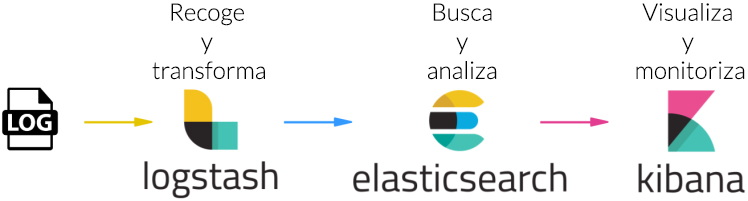
\includegraphics[width=1\linewidth]{img/elk.jpg}
    \caption{Arquitectura del sistema ELK.}
    \label{fig:elk}
\end{figure}

\apendice{Documentación técnica de programación}

Poder replicar experimentos, versiones de programas, con que datos se hacen, de donde los he sacado, comentar código

\section{Introducción}
En este anexo se va a explicar todo lo necesario que tiene que saber un programador para poder replicar los experimentos de este estudio. Incluyendo versiones de los programas usados, origen de las fuentes de datos así como la estructura del código desarrollado. 

\section{Estructura de directorios}
El proyecto se estructura en una serie de directorios que contienen tanto la documentación como el material empleado en cada escenario desarrollado.
\begin{itemize}
    \item \textbf{docs}: contiene toda la información relacionada con la documentación del proyecto, como pueden ser PDFs, ficheros LaTeX o fuentes e imágenes empleadas.
    \item \textbf{Escenario 1: ingesta desde fichero en Elastic}: contiene tanto los archivos involucrados en este escenario como el \textit{dashboard} final del mismo.
    \item \textbf{Escenario 2: ingesta desde fichero con Logstash}: contiene tanto los archivos involucrados en este escenario como el \textit{dashboard} final del mismo.
    \item \textbf{Escenario 3: ingesta a través de WebSocket a Elastic}: contiene el script de ingesta de datos junto con el \textit{dashboard} final obtenido.
    \item \textbf{Escenario 4: ingesta a través de WebSocket con Logstash}: contiene el script de ingesta de datos y el archivo de configuración de Logstash junto con el \textit{dashboard} final obtenido.
    \item \textbf{Escenario 5: ingesta de data stream con MapReduce en el servidor mediante Logstash}: contiene los scripts de ingesta de datos y el archivo de configuración de Logstash junto con el \textit{dashboard} final obtenido.
    \item \textbf{Machine Learning}: contiene los scripts de ingesta de datos junto con el \textit{dashboard} final obtenido.

\end{itemize}

\section{Manual del programador}
Para el desarrollo del proyecto se han empleado una serie de programas a parte de los que conforman el ecosistema ELK. En este apartado se van a exponer las características y configuraciones empleadas en cada uno de ellos para el desarollo del proyecto.

\subsection{ElasticSearch}
Este programa se descargó desde la \href{https://www.elastic.co/es/elasticsearch}{página oficial} del software, instalando la versión 8.11.3, la cuál consiste en un archivo comprimido el cuál una vez descomprimido ya permite el uso mediante la ejecución del archivo \textit{elasticsearch.bat} alojado en el directorio \textit{bin}, el cuál si es ejecutado arrancará el servidor en el equipo, y tras unos segundos permitirá consultar su estado accediendo desde el navegador al puerto 9200, en el cuál estará corriendo el servidor de Elastic \ref{fig:elastic9200}.

\begin{figure}
    \centering
    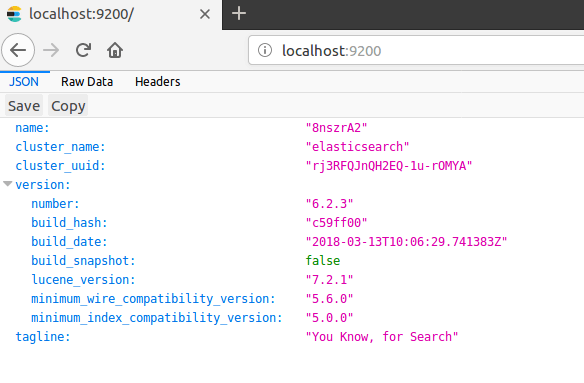
\includegraphics[width=1\linewidth]{img/elastic.png}
    \caption{ElasticSearch corriendo en el puerto local 9200}
    \label{fig:elastic9200}
\end{figure}

\subsection{Logstash}
Esta herramienta de administración de datos fue descargada desde la \href{https://www.elastic.co/es/logstash}{página oficial de Logstash}, en la versión 8.13.2, que al igual que el anterior, consistirá en un comprimido que una vez extraído se tendrá que crear un archivo de tipo .conf que será la configuración que empleará Logstash en el momento de ejecución del archivo logstash.bat ubicado en la carpeta \textit{bin}. Una vez tenemos el archivo de configuración listo ejecutaremos desde la terminal el archivo .bat mencionado anteriormente indicándole la configuración que seguirá.

\subsection{Kibana}
El útimo componente del \textit{stack ELK}, al igual que los otros dos, ha sido descargado desde la \href{https://www.elastic.co/es/kibana}{página oficial} del programa, en la versión 8.11.3, y que una vez extraído el archivo comprimido, se ejecutará el archivo \textit{kibana.bat} alojado en el directorio \textit{bin}, el cuál al ser ejecutado arrancará el programa, y tras unos segundos permitirá acceder al mismo desde el navegador en el puerto 5601, en el cuál estará corriendo el servicio de Kibana. 

\subsection{Python}
Fue instalado en su momento a través la \href{https://www.python.org/}{página oficial} con la versión 3.12.2, la cuál consiste en un ejecutable que una vez abierto instalará todos los archivo necesarios para poder escribir y ejecutar código en este lenguaje de programación.

\subsection{Jupyter Notebook}
Este programa fue descargado desde la \href{https://jupyter.org/}{página del proyecto Jupyter}, en la cuál se ofrecen diferentes programas de la empresa. en la versión 7.1.2. Una vez instalado el programa, desde la terminal se ejecuta el comando \textit{jupyter notebook} y en el puerto local 8888 se mostrará la estructura de directorios del servicio.

\subsection{Visual Studio Code}
El software que se usó para programar parte del código empleado en el proyecto fue descargado desde la \href{https://code.visualstudio.com/}{página oficial} del programa en la versión 1.90.2, y una vez ejecutado el instalador el programa estará listo para ser usado.

\section{Compilación, instalación y ejecución del proyecto}
Una vez se tiene todo el software instalado y listo, es necesario descargar los datos utilizados en el proyecto. Para ello, se deja a disposición el \href{https://github.com/hds1001/Estudio-y-configuracion-de-un-sistema-ELK}{repositorio del proyecto} en el cuál se encuentra toda la información empleada con la estructura de directorios mencionada anteriormente.

En este apartado vamos a desarrollar escenario por escenario el funcionamiento del mismo, pero lo primero antes de iniciar con el primero de ellos es tener corriendo tanto ElasticSearch como Kibana de la manera que se ha mencionado antes. Una vez la terminal muestra que ambos programas están en ejecución, se puede empezar a trabajar.

\subsection{Escenario 1: ingesta desde fichero en Elastic}
En este primer escenario, se empleó como origen de los datos un \textit{dataset} conocido en el mundo de la ciencia de datos, como es el de los pasajeros del desastre del Titanic. Este fue obtenido desde el \href{https://github.com/datasciencedojo/datasets/blob/master/titanic.csv}{repositorio} de datos \textit{Data Science Dojo}, el cuál pone a disposición pública gran variedad de \textit{datasets} para experimentar.

El \textit{dataset} consiste en un archivo de valores separados por comas con información de los 891 pasajeros del Titanic \ref{fig:titanic}, incluyendo campos como la clase del pasajero, su nombre o su edad entre otros.

\begin{figure}
    \centering
    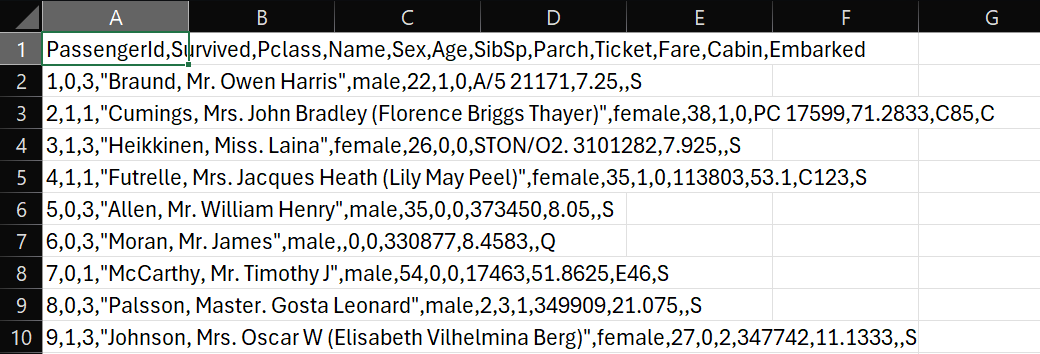
\includegraphics[width=1\linewidth]{titanic.png}
    \caption{\textit{Dataset} del titanic.}
    \label{fig:titanic}
\end{figure}

Una vez se tiene en el sistema el archivo \textit{titanic.csv}, el siguiente paso teniendo en movimiento tanto Elastic como Kibana, es importar el archivo a ElasticSearch a través de la opción \textit{Upload a file} \ref{fig:escenario11}.

\begin{figure}
    \centering
    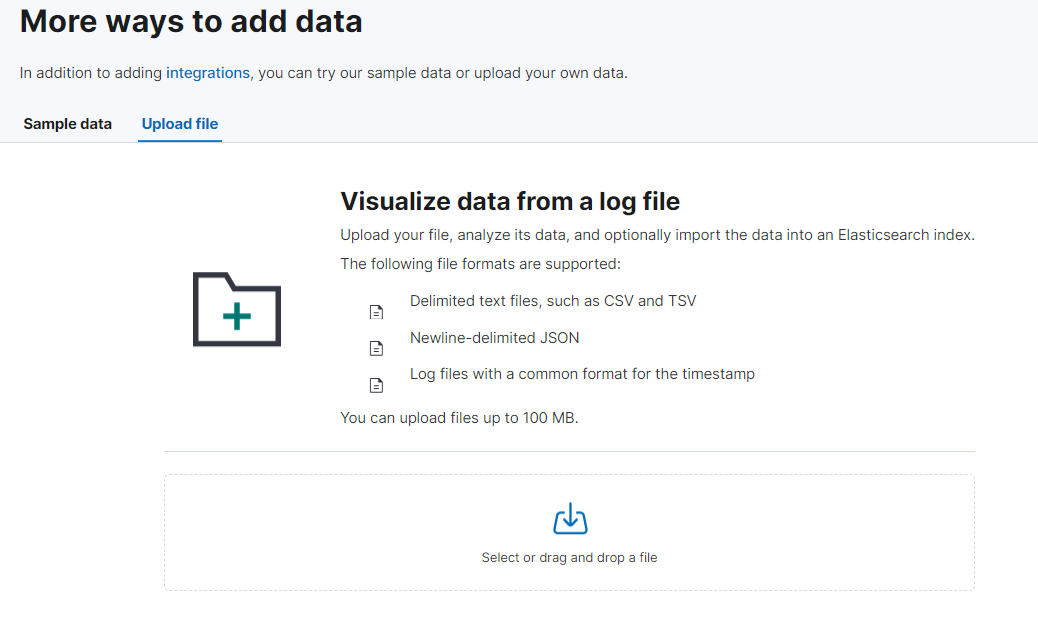
\includegraphics[width=1\linewidth]{img/ingesta1.png}
    \caption{Pantalla para importar datos del primer escenario.}
    \label{fig:escenario11}
\end{figure}

Cuando el fichero se haya cargado en ElasticSearch, se podrá comprobar desde Kibana en el apartado \textit{Discover} que todos los datos han sido cargados correctamente. Esta parte del proceso queda explicada con detenimiento en el anexo \textit{Manual de Kibana}.

\paragraph{}

\subsection{Escenario 2: ingesta desde fichero con Logstash}
Para este segundo escenario se requiere del uso de Logstash para transformar y cargar en Elastic un fichero presente en el sistema. El origen de la fuente de datos de este fichero va a ser el archivo \textit{casas.log} \ref{fig:casas}, un conjunto de datos sobre los diferentes inmuebles que se ofertan en una inmobiliaria, con información como la ciudad, el barrio o el precio entre otros.
\begin{figure}
    \centering
    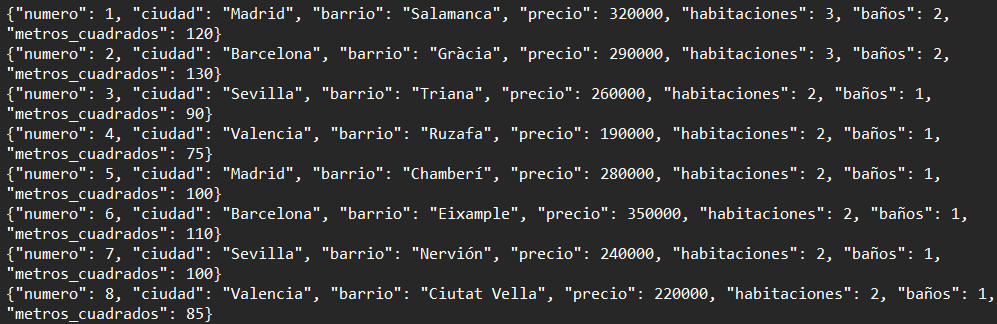
\includegraphics[width=1\linewidth]{img/casas.png}
    \caption{Estructura del fichero fuente de datos del segundo escenario.}
    \label{fig:casas}
\end{figure}

Una vez están en ejecución los otros dos componentes del \textit{stack ELK}, hay que poner en funcionamiento Logstash, pero primero se necesita un archivo que indique la configuración a seguir en este escenario, y ese va a ser el archivo \textit{escenario2.conf}, el cuál estará estructurado de manera que en el apartado \textit{input} \ref{fig:input2} se indique el \textit{path} hacia el archivo \textit{casas.log}, en la sección de filtrado \ref{fig:filter2} del archivo de configuración se realizará un mutado de los datos como se explicó en la documentación de la memoria, y en la parte de salida de los datos \ref{fig:output2} se especifica el destino, que es Elastic.

\begin{figure}
    \centering
    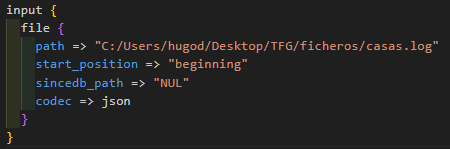
\includegraphics[width=1\linewidth]{img/input2.png}
    \caption{Apartado \textit{input} del archivo de configuración del segundo escenario.}
    \label{fig:input2}
\end{figure}

\begin{figure}
    \centering
    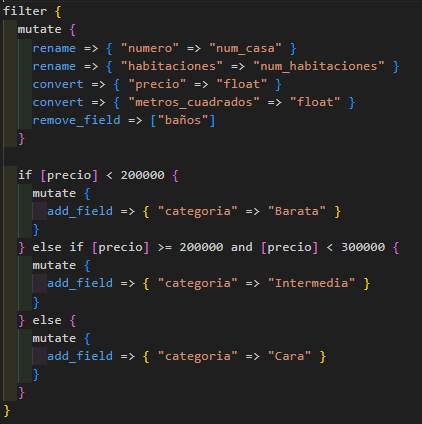
\includegraphics[width=1\linewidth]{img/filter2.png}
    \caption{Apartado \textit{filter} del archivo de configuración del segundo escenario.}
    \label{fig:filter2}
\end{figure}

\begin{figure}
    \centering
    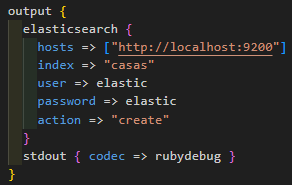
\includegraphics[width=1\linewidth]{img/output2.png}
    \caption{Apartado \textit{output} del archivo de configuración del segundo escenario.}
    \label{fig:output2}
\end{figure}

Una vez se tiene listo el archivo de configuración, desde la terminal habrá que dirigirse a la carpeta que contiene el archivo \textit{logstash-bat}, que es el directorio \textit{bin}, y desde ahi especifacar cuál es la configuración que se quiere usar en el momento de ejecución mediante el comando \textit{logstash -f escenario2.conf}. Al ejecutar se mostrarán por pantalla los datos modificados y llegarán a Elastic en dirección al índice \textit{casas}, el cuál podrá ser consultado más adelante como se indica en el \textit{Manual de Kibana}.

\paragraph{}

\subsection{Escenario 3: ingesta a través de WebSocket a Elastic}
En este tercer escenario, el origen de la ingesta de datos será un script que se suscribirá a un envío de datos en vivo por parte de la plataforma de criptodivisas \href{https://finnhub.io/docs/api/websocket-trades}{\textit{Finnhub}}. Esta suscripción se realiza a través de un WebSocket programado en Python.

Para la ejecución de este script será necesario la importación de las librerías \textit{websocket}, \textit{elasticsearch}, \textit{datetime} y \textit{json} al principio del código. Una vez importadas, en la primera parte del código\ref{fig:escenario31}, se especifica en la variable \textit{client} la dirección del puerto en el que se ejecuta el servidor de ElasticSearch. Tras esto, el método \textit{on message} define que el contenido del mensaje que se va a mandar está en formato JSON e incluirá la fecha en la que fue mandado. También indica que el contenido será mandado al índice \textit{websockets data}.
\begin{figure}
    \centering
    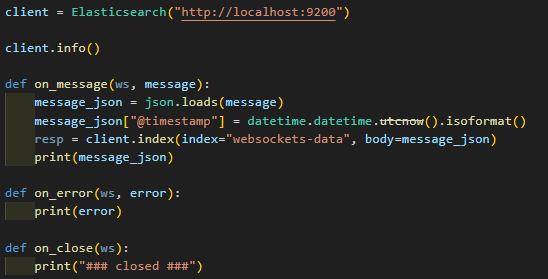
\includegraphics[width=1\linewidth]{img/escenario31.png}
    \caption{Primera parte del script de carga del tercer escenario.}
    \label{fig:escenario31}
\end{figure}

Comenzando con la segunda parte del código\ref{fig:escenario32}, en el método \textit{on open} se definen las divisas cuyo contenido va a ser incluído en el mensaje mandado a Elastic. Tras esto se define el método \textit{main} en el cuál se especificará la key de la API de \textit{Finnhub} utilizada como suscripción. También se especifica que mientrás el script esté operativo se sigan mandando datos hasta que se detenga.
\begin{figure}
    \centering
    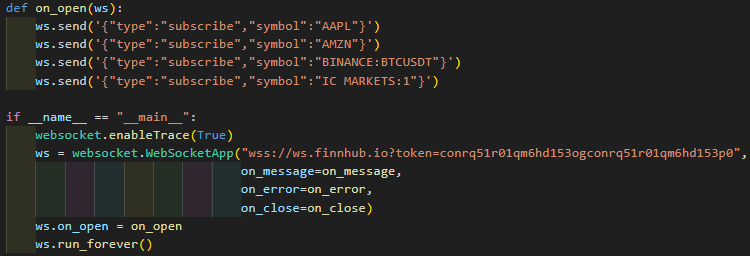
\includegraphics[width=1\linewidth]{img/escenario32.png}
    \caption{Segunda parte del script de carga del tercer escenario.}
    \label{fig:escenario32}
\end{figure}

Este script es la piedra angular de este escenario, ya que tras su ejecución los datos llegarán a Elastic y serán mostrados en el \textit{dashboard} correspondiente tal y como se mencionó en la documentación de la memoria.

\subsection{Escenario 4: ingesta a través de WebSocket con Logstash}

Para este cuarto escenario, el origen de la fuente de datos será el mismo que en el tercero, peró habrá una serie de cambios en el script de carga, de manera que en lugar de los datos ser mandados directamente un índice de ElasticSearch, serán mandado a Logstash donde se procesarán y cargarán en Elastic.

La primera parte del script de carga de datos \ref{fig:escenario41} está formada por la importación de las librerías \textit{requests}, \textit{json} y \textit{websocket}, y por el método de renombrado de campos mandados por \textit{Finnhub}, de manera que el campo que llega como \textit{s} sea mandado como \textit{Symbol}, el que llega como \textit{p} sea mandado como \textit{LastPrice}, el que llega como \textit{t} sea mandado como \textit{Timestamp}, el que llega como \textit{v} sea mandado como \textit{Volume}, y el que llega como \textit{c} sea mandado como \textit{TradeConditions} a Logstash.

\begin{figure}
    \centering
    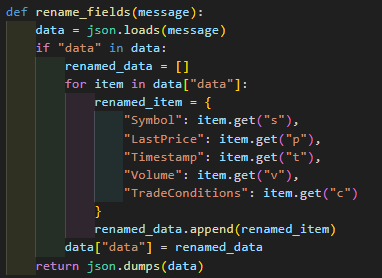
\includegraphics[width=1\linewidth]{img/websocket1.png}
    \caption{Primera parte del script de carga del cuarto escenario.}
    \label{fig:escenario41}
\end{figure}

En la segunda parte del script de carga de datos \ref{fig:escenario42}, se define el método \textit{on message} el cuál especifica que los datos serán mandados en formato JSON al puerto local 8080 en el cuál estará escuchando Logstash a la espera de información. También se definen los métodos \textit{on error} y \textit{on close} que son meramente informativos de cara la visualización del envío de datos en la terminal.
\begin{figure}
    \centering
    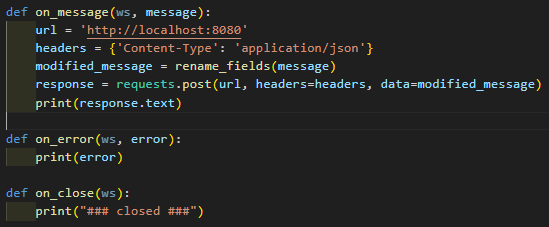
\includegraphics[width=1\linewidth]{img/websocket2.png}
    \caption{Segunda parte del script de carga del cuarto escenario.}
    \label{fig:escenario42}
\end{figure}

Para la tercera y última parte del script de carga de datos \ref{fig:escenario43}, en el método \textit{on open} se definen las divisas que se mandarán a Logstash, y en el método \textit{main} se especifica la \textit{key} empleada como suscripción al servicio de envío de datos que ofrece \textit{Finnhub}.

\begin{figure}
    \centering
    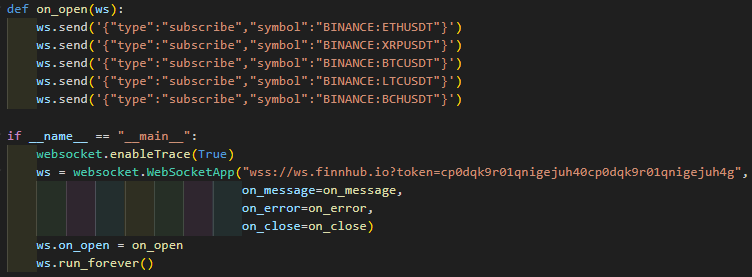
\includegraphics[width=1\linewidth]{img/websocket3.png}
    \caption{Tercera parte del script de carga del cuarto escenario.}
    \label{fig:escenario43}
\end{figure}
Una vez se ejecuta el script los datos serán mandados en forma \textit{raw} \ref{fig:salida1} al puerto local 8080, donde Logstash está a la espera de recibir datos. Una vez son mandados allí, pasan por el filtro especificado en el archivo de configuración de este cuarto escenario, el cuál esta conformado por dos partes. En la primera parte del apartado de filtrado del archivo de configuración \ref{fig:filtrado1}, se especifica que la información que va a llegar va a estar en formato JSON, que el campo \textit{TradeConditions} va a ser eliminado del mensaje final, y que el tipo del campo \textit{LastPrice} será \textit{float}, que \textit{Timestamp} será \textit{integer} y \textit{Volume} será \textit{float}.

\begin{figure}
    \centering
    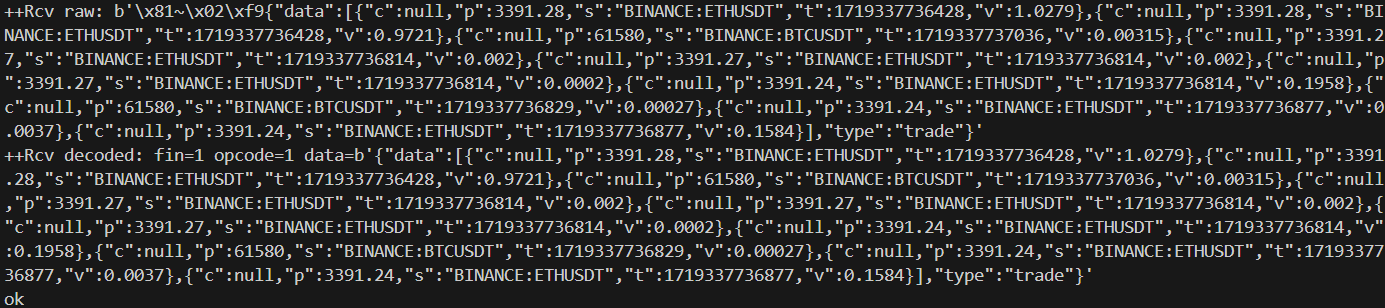
\includegraphics[width=1\linewidth]{img/salida1.png}
    \caption{Salida por pantalla de los datos del script del cuarto escenario.}
    \label{fig:salida1}
\end{figure}


\begin{figure}
    \centering
    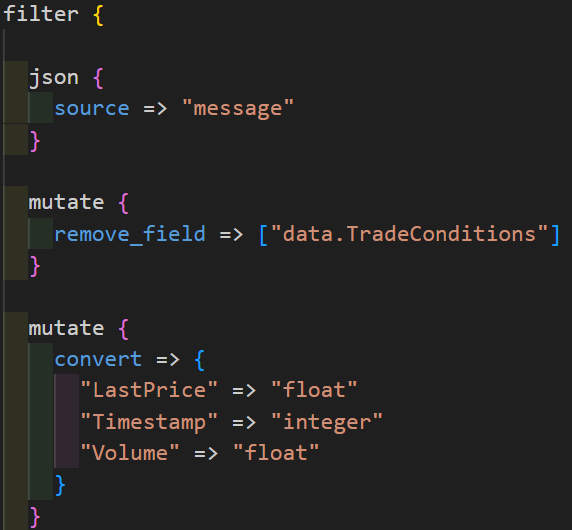
\includegraphics[width=0.5\linewidth]{escenario41.png}
    \caption{Primera parte del filtrado del archivo de configuración del cuarto escenario.}
    \label{fig:filtrado1}
\end{figure}


En la parte final del filtrado del archivo de configuración \ref{fig:filtrado2}, una vez se tienen modificados los tipos de los campos \textit{LastPrice} y \textit{Volume}, en lenguaje \textit{Ruby} se ha programado la inserción de un nuevo campo \textit{TotalPrice} calculado a partir del producto de estos dos campos.
\begin{figure}
    \centering
    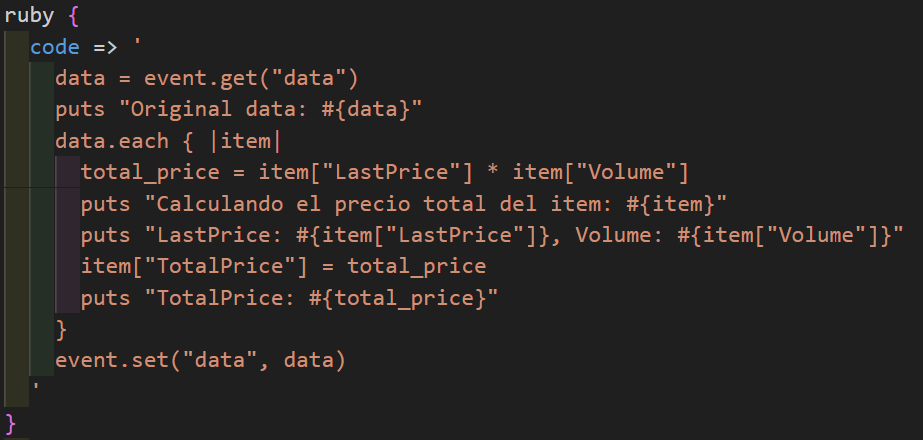
\includegraphics[width=1\linewidth]{img/escenario42.png}
    \caption{Segunda parte del filtrado del archivo de configuración del cuarto escenario.}
    \label{fig:filtrado2}
\end{figure}

Habiendo finalizado el archivo de configuración, se tienen en ejecución tanto Logstash como el script, los datos se irán mandando a Elastic con una estructura más entendible \ref{fig:salida2}.

\begin{figure}
    \centering
    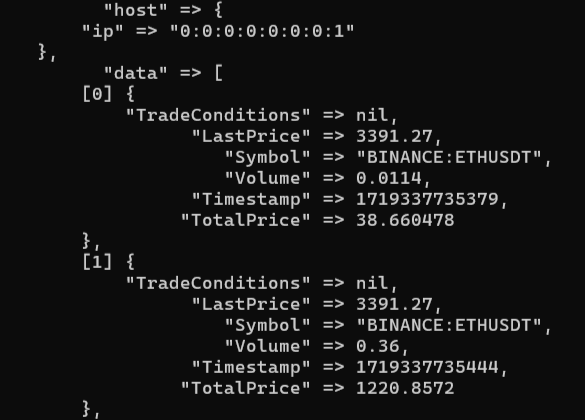
\includegraphics[width=1\linewidth]{img/salida2.png}
    \caption{Salida por pantalla de los datos una vez salen de Logstash hacia Elastic.}
    \label{fig:salida2}
\end{figure}
\paragraph{}
\paragraph{}
\paragraph{}
\paragraph{}
\paragraph{}
\paragraph{}
\paragraph{}



\subsection{Escenario 5: ingesta de data stream con MapReduce en el servidor mediante Logstash}

En este quinto escenario se pretende aplicar MapReduce a datos en vivo generados a través de un script que irá añadiendo líneas a un fichero llamado \textit{test.log} que Logstash irá leyendo y actualizando el envío de sus datos a Elastic. Este fichero contendrá información sobre las transacciones que se han hecho en un negocio, incluyendo información como el identificador del cliente, el método de pago o la categoría del producto comprado.

En la primera parte de este script generador de datos se especifica tanto la ruta del fichero destino de los datos generados, como los valores sobre los que irá operando el método generador de los datos. Para la ejecución de este script hará falta la importación de las librerías \textit{json}, \textit{random}, \textit{time} y \textit{datetime}.
\begin{figure}
    \centering
    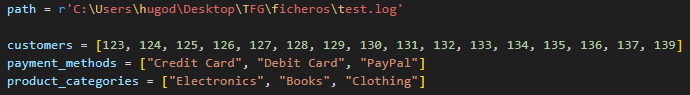
\includegraphics[width=1\linewidth]{img/escenario51.png}
    \caption{Primera parte del generador de datos del quinto escenario.}
    \label{fig:generador1}
\end{figure}

El método \textit{generate transaction} es el encargado de generar elecciones aleatorias sobre las que se han especificado previamente para los campos \textit{customer id}, \textit{amount}, \textit{payment method} y \textit{product category}. También indicará que cada línea escrita en el archivo contendrá estos campos junto a un identificador de la transacción y la fecha en la que fue generado.
\begin{figure}
    \centering
    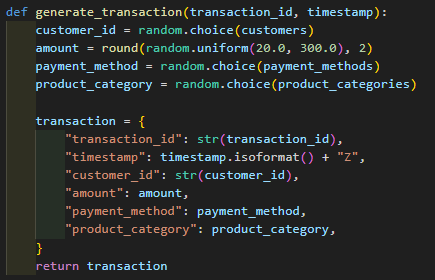
\includegraphics[width=1\linewidth]{img/escenario52.png}
    \caption{Segunda parte del generador de datos del quinto escenario.}
    \label{fig:generador2}
\end{figure}

En esta última parte del script se establece un bucle en el que comenzando por la transacción número 1 se irán generando transacciones cada segundo, y no se detendrá hasta que se pare el script.
\begin{figure}
    \centering
    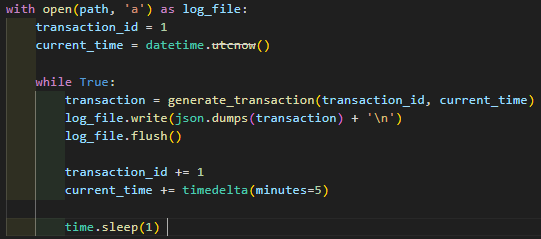
\includegraphics[width=1\linewidth]{img/escenario53.png}
    \caption{Tercera parte del generador de datos del quinto escenario.}
    \label{fig:generador3}
\end{figure}

Con esto, una vez se ejecuta el script, resultará en que el archivo \textit{test.log} irá almacenando las transacciones en un formato entendible tanto para el usuario como para Logstash.

\begin{figure}
    \centering
    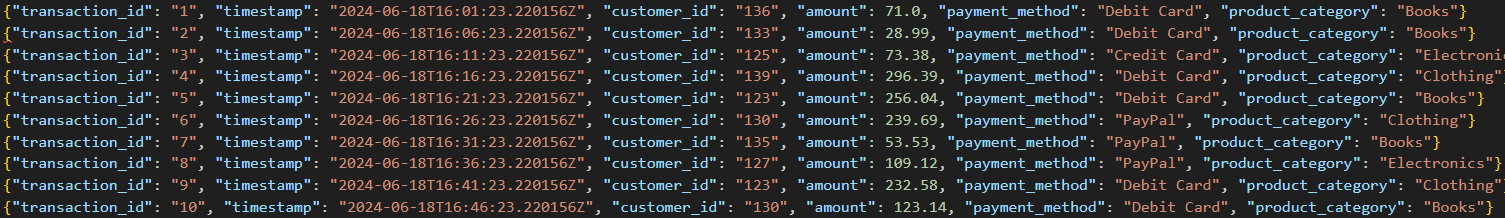
\includegraphics[width=1\linewidth]{img/salida3.png}
    \caption{Estructura de la fuente de los datos del quinto escenario.}
    \label{fig:salida3}
\end{figure}

Cuando el archivo se va llenando de líneas, se tiene Logstash en ejecución simultáneamente, de manera que se vaya ejecutando el método \textit{aggregate} tal y como se explicó en la documentación de la memoria.

\paragraph{}
\paragraph{}
\paragraph{}
\paragraph{}
\paragraph{}
\paragraph{}
\paragraph{}
\paragraph{}
\paragraph{}
\paragraph{}
\paragraph{}
\paragraph{}
\paragraph{}
\paragraph{}


\subsection{Machine Learning}

En este último caso planteado en el cuál se aplica una serie de algoritmos que ofrece la librería SKLearn sobre el popular \textit{dataset} Iris, la manera de ingestar los datos se planteó de manera que los datos de Iris estuvieran presentes en un índice en Elastic, estos datos se cargarán en el script que aplica los algoritmos, y una vez cargados cada algoritmo devolverá los datos procesados a un índice individual para cada uno.

Para resolver esta estructura planteada, se generaron dos scripts. En el primero de ellos se crea un índice en Elastic que contiene el \textit{dataset} Iris. Son necesarias las librerías \textit{pandas}, \textit{sklearn} y \textit{elasticsearch}. De manera que inicialmente se cargan los datos de Iris tal cuál viene de SKLearn, con el mismo nombre de los campos (esto va a ser importante en el segundo script para realizar operaciones sobre ellos) \ref{fig:script11}. También se establece la conexión con ElasticSearch indicando el puerto local en el que se ubica el servidor.

\begin{figure}
    \centering
    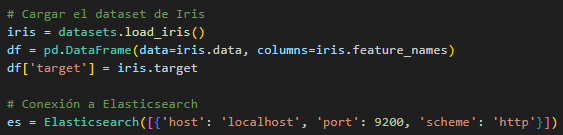
\includegraphics[width=1\linewidth]{img/iris1.png}
    \caption{Parte inicial del primer script de Machine Learning.}
    \label{fig:script11}
\end{figure}

En la segunda parte del primer script se va a definir tanto el nombre del índice que contendrá el \textit{dataset} Iris como el nombre de las propiedas del mismo junto con el tipo que son \ref{fig:script12}, de manera que coincidan con las del \textit{dataset} original para que no haya errores. 

\begin{figure}
    \centering
    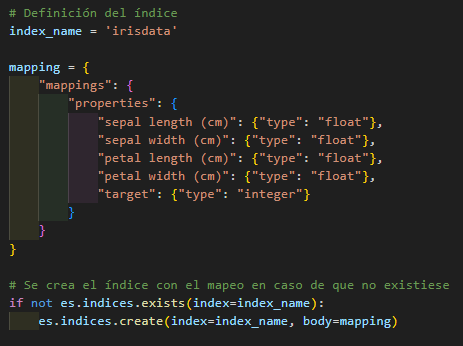
\includegraphics[width=1\linewidth]{img/iris2.png}
    \caption{Segunda parte del primer script de Machine Learning}
    \label{fig:script12}
\end{figure}

Una vez se tiene toda la información del destino de los datos cargada, se procede al envío de los mismos \ref{fig:script13} de manera que se vayan mostrando por pantalla en la terminal a medida que van siendo cargados.

\begin{figure}
    \centering
    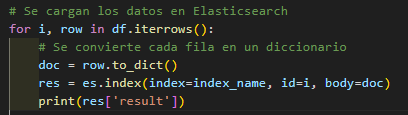
\includegraphics[width=1\linewidth]{img/iris3.png}
    \caption{Parte final del primer script de Machine Learning.}
    \label{fig:script13}
\end{figure}

\paragraph{}
\paragraph{}
\paragraph{}
\paragraph{}


Tras ejecutar este primer script los datos ya están presentes en Elastic, y para fragmentar el trabajo se creó un segundo script en el que se trabajara sobre esos datos cargados. En este segundo script lo primero que se hacer es definir tanto la función \textit{load data from elasticsearch} como \textit{create index} que lo que van a hacer es facilitar la carga de datos del índice que se le indique pasado por valor, y crear nuevos índices con los nombres indicados \ref{fig:script21}. Están son funciones auxiliares en futuros pasos del script.


\begin{figure}
    \centering
    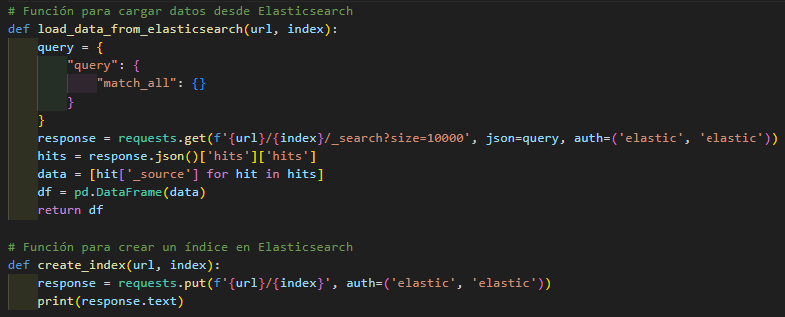
\includegraphics[width=1\linewidth]{img/iris4.png}
    \caption{Definición de funciones auxiliares para el segundo script de Machine Learning.}
    \label{fig:script21}
\end{figure}

En la segunda parte del script se van a seguir realizando operaciones auxiliares para poder operar con los algoritmos. Se establece la URL y el nombre del índice a cargar, que es el mismo en el que se ingestaron los datos de Iris en el script previo, de manera que los datos sean cargados y separados para poder trabajar sobre ellos. También se generan los distintos índices que contendrán los datos obtenidos como resultado de la ejecución de cada algoritmo.

\begin{figure}
    \centering
    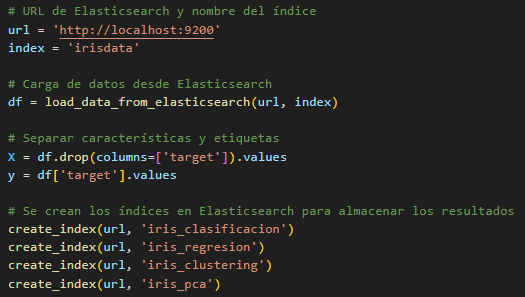
\includegraphics[width=1\linewidth]{img/iris5.png}
    \caption{Definición de operaciones auxiliares y carga de datos para el segundo script de Machine Learning.}
    \label{fig:script22}
\end{figure}

Una vez está toda la información cargada y lista para ser usada, se comienza por el primer algoritmo utilizado, que va a ser uno de clasificación, concretamente \textit{KNN} o K vecinos más cercanos, en el cuál mediante los métodos proporcionados por SKLearn como \textit{train test split}  o \textit{fit}, se creará y entrenará un clasificador en función de los tres vecinos más cercanos \ref{fig:clasificacion1}, obteniendo así una precisión para este clasificador la cuál será exportada a Elastic así como todos los datos que se han procesado en la ejecución del algoritmo, que irán destinados al índice \textit{iris clasificacion} para su posterior uso y exposición en Kibana \ref{fig:clasificacion2}. 

\begin{figure}
    \centering
    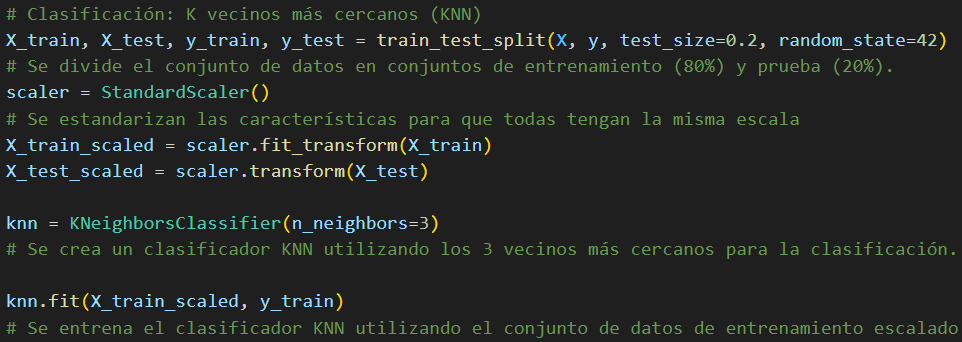
\includegraphics[width=1\linewidth]{img/iris6.png}
    \caption{Generación del clasificador y entrenamiento.}
    \label{fig:clasificacion1}
\end{figure}
\begin{figure}
    \centering
    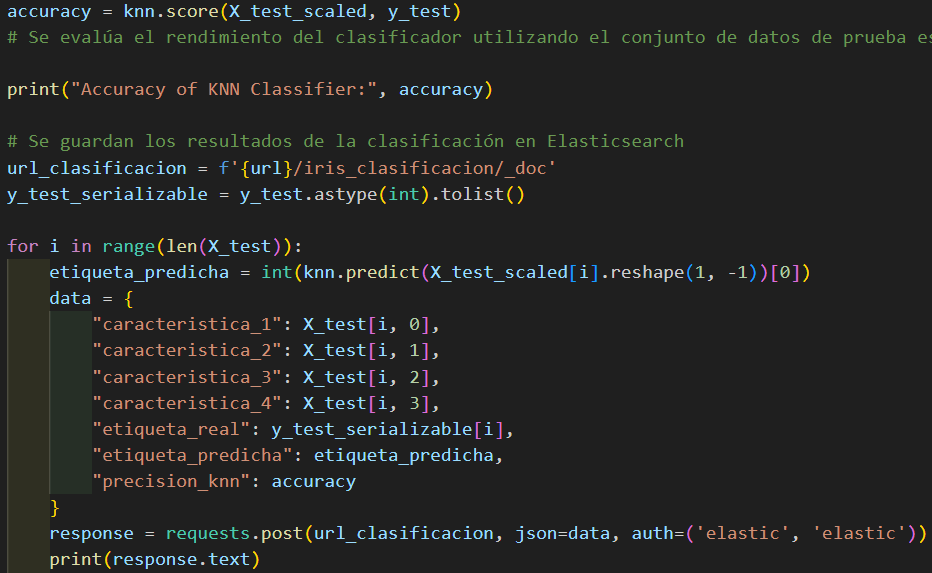
\includegraphics[width=1\linewidth]{img/iris7.png}
    \caption{Cálculo de la precisión del clasificador y envío de datos a Elastic.}
    \label{fig:clasificacion2}
\end{figure}

El siguiente algoritmo al que se le ha dado uso es el de regresión lineal, en el cuál tomando como referencia la tercera característica (longitud del pétalo) para el eje X, y la cuarta característica (anchura del pétalo) para el eje Y, se cree un modelo que sea capaz de predecir un comportamiento típico de los datos. Para ello se le entrena mediante el método \textit{fit} con un conjunto de datos de entrenamiento obtenido de los totales \ref{fig:regresion1}. Posteriormente se evalúa su rendimiento y se manda a Elastic junto con el resto de datos empleados al índice \textit{iris regresion} r\ref{fig:regresion2}.
\begin{figure}
    \centering
    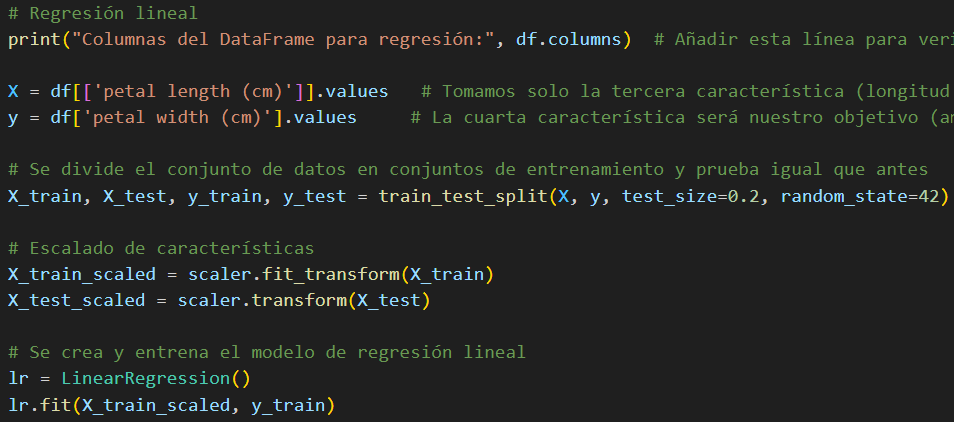
\includegraphics[width=1\linewidth]{img/iris8.png}
    \caption{Generación del modelo de regresión y los conjuntos de entrenamiento.}
    \label{fig:regresion1}
\end{figure}


\begin{figure}
    \centering
    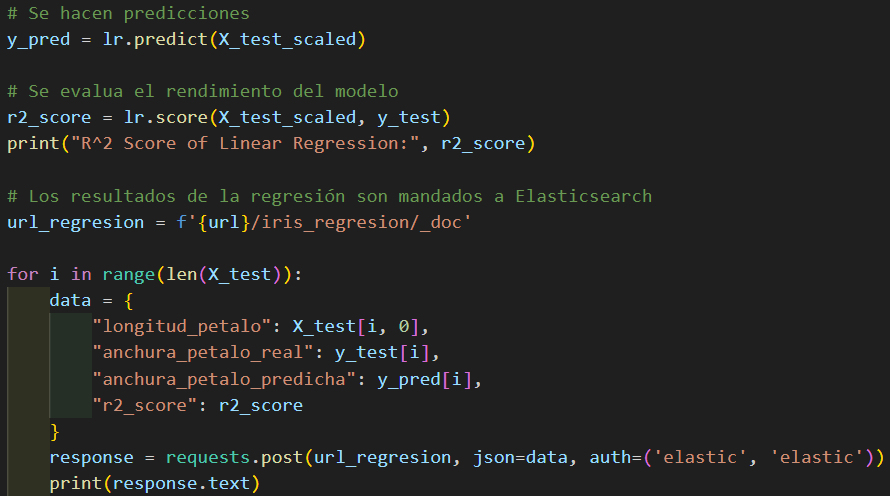
\includegraphics[width=1\linewidth]{img/iris9.png}
    \caption{Cáclulo del rendimiento del modelo y envío de datos a Elastic.}
    \label{fig:regresion2}
\end{figure}


En este tercer algoritmo se va a emplear uno de \textit{clustering}, el \textit{K Means}, en el cuál se van a generar tres clusters de manera que se cree un modelo que devuelva una visualización de los tres en forma de gráfico de dispersión de la longitud y anchura de los sépalos \ref{fig:cluster1}. Una vez se obtiene el gráfico, los datos son mandados a Elastic para poder visualizarlos en un \textit{dashboard}.
\begin{figure}
    \centering
    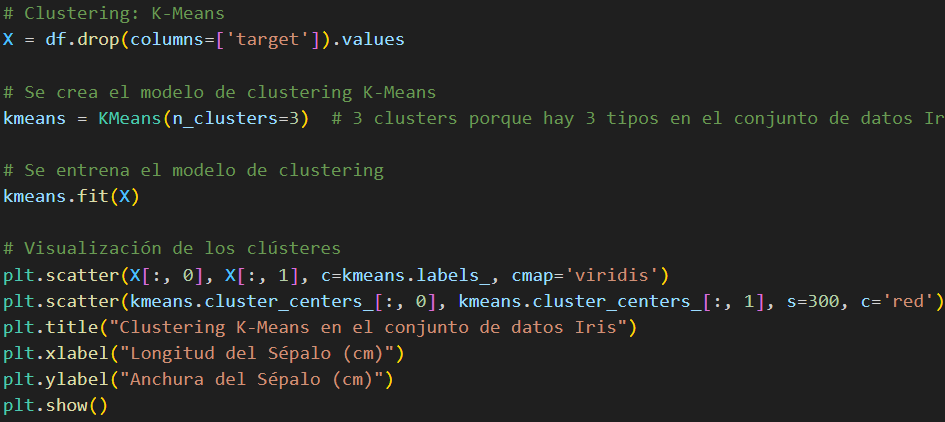
\includegraphics[width=1\linewidth]{img/iris10.png}
    \caption{Estructura del algoritmo \textit{K Means} del segundo script de Machine Learning.}
    \label{fig:cluster1}
\end{figure}

\paragraph{}
\paragraph{}
\paragraph{}

Por último se va a hacer uso de otro algoritmo visual de reducción de dimensionalidad, \textit{PCA}. Al igual que en el anterior, se quiere generar un gráfico bidimensional, por lo que se toman dos componentes equivalentes a los pétalos y sépalos distinguidos por el campo \textit{target} \ref{fig:pca1}. Se entrena el modelo y se genera un gráfico de dispersioón con estos dos componentes el cuál será enviado a Elastic junto con toda la información involucrada. 
\begin{figure}
    \centering
    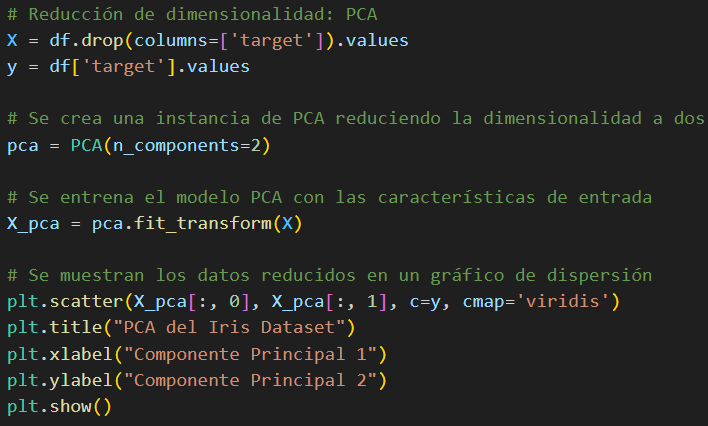
\includegraphics[width=1\linewidth]{img/iris11.png}
    \caption{Estructura del algoritmo de reducción de la dimensionalidad del segundo script de Machine Learning.}
    \label{fig:pca1}
\end{figure}

Tras ejecutar los dos scripts los datos llegarán los diferentes índices que se han ido indicando en ambos. El \textit{dataset} Iris estará almacenado en el índice \textit{irisdata} \ref{fig:index1}, los datos del algoritmo de clasificiación en el índice \textit{iris clasificacion} \ref{fig:index2}, los datos del algoritmo de regresión en el índice \textit{iris regresion} \ref{fig:index3}, los datos del algoritmo de clustering en el índice \textit{iris clustering} \ref{fig:index4},  y por último los datos del algoritmo de reducción de dimensionalidad en el índice \textit{iris pca} \ref{fig:index5}.

\begin{figure}
    \centering
    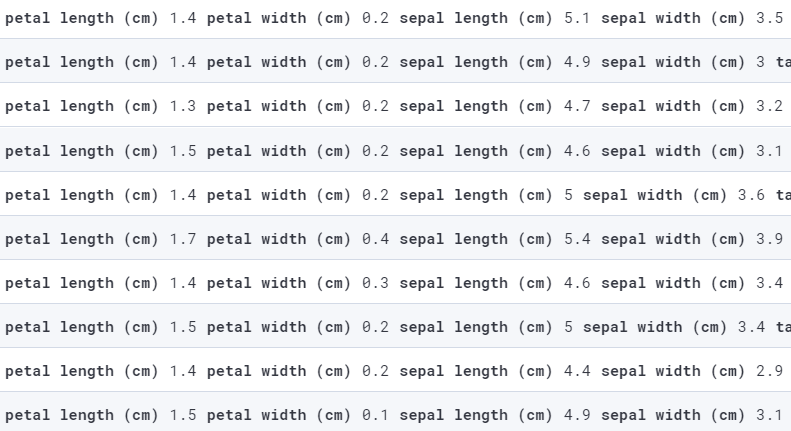
\includegraphics[width=1\linewidth]{img/iris13.png}
    \caption{Índice \textit{irisdata} con información de los datos de Iris.}
    \label{fig:index1}
\end{figure}


\begin{figure}
    \centering
    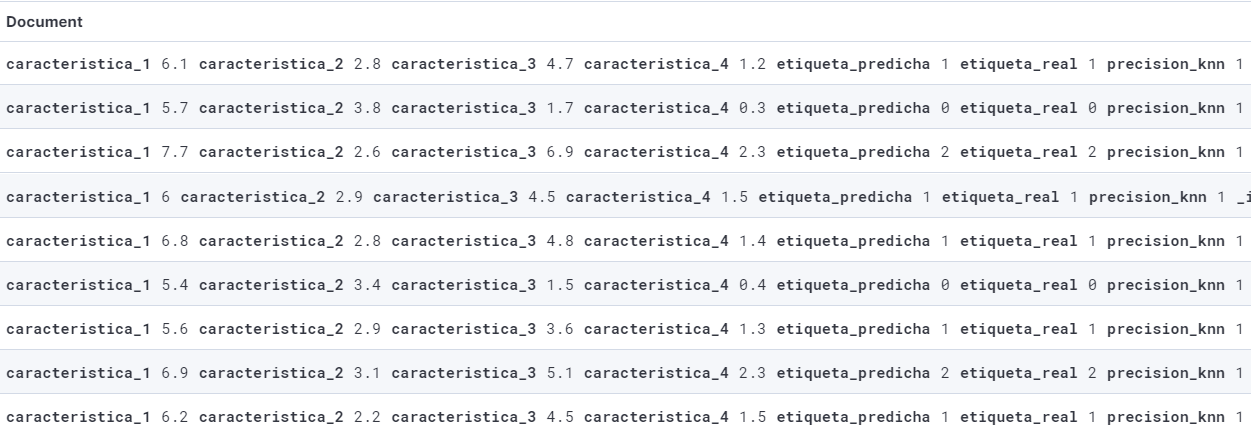
\includegraphics[width=1\linewidth]{img/iris14.png}
    \caption{Índice \textit{iris clasificacion} con información de los datos procesados por el algoritmo de clasificación.}
    \label{fig:index2}
\end{figure}


\begin{figure}
    \centering
    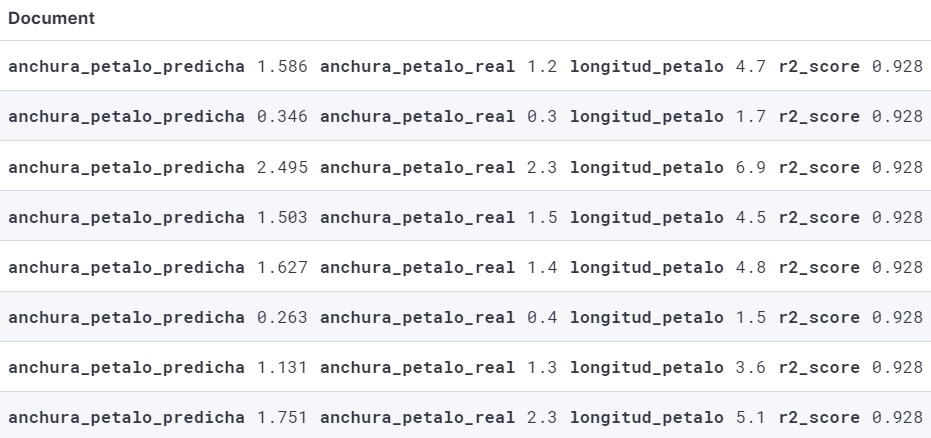
\includegraphics[width=1\linewidth]{img/iris15.png}
    \caption{Índice \textit{iris regresion} con información de los datos procesados por el algoritmo de regresión.}
    \label{fig:index3}
\end{figure}


\begin{figure}
    \centering
    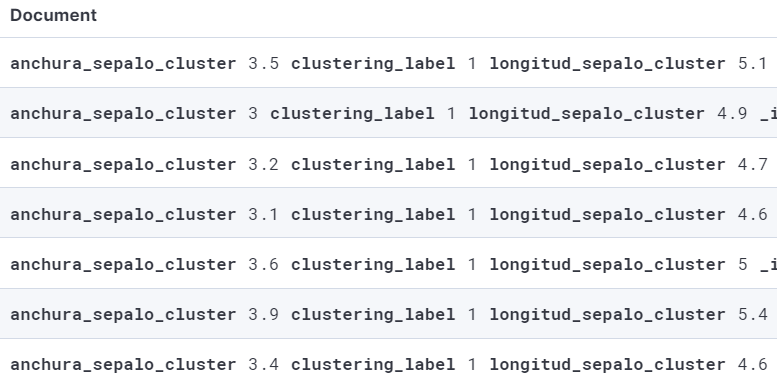
\includegraphics[width=1\linewidth]{img/iris16.png}
    \caption{Índice \textit{iris clustering} con información de los datos procesados por el algoritmo de clustering.}
    \label{fig:index4}
\end{figure}



\begin{figure}
    \centering
    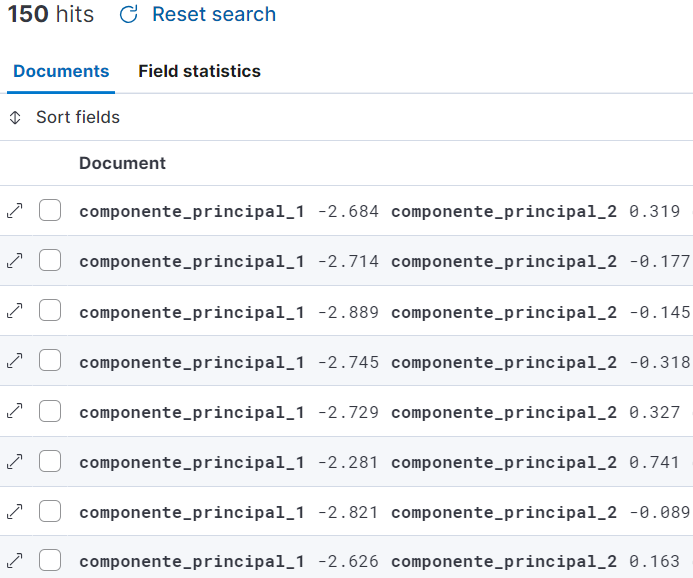
\includegraphics[width=1\linewidth]{img/iris17.png}
    \caption{Índice \textit{iris pca} con información de los datos procesados por el algoritmo de reducción de dimensionalidad.}
    \label{fig:index5}
\end{figure}










\apendice{Manual de Kibana}

\section{Introducción}
Este anexo en un TFG convencional recibiría el nombre de \textit{Manual de usuario}, pero al consistir este TFG de un estudio, se ha decidido modificarlo a \textit{Manual de Kibana}, y se indagará en todas las posibilidades y caracterísiticas avanzas que ofrece el programa más visual e intuitivo de los tres componentes del stack ELK. 

\section{Requisitos de usuarios}
Este \textit{software} no requiere de gran cantidad de requisitos ni es muy demandante en recursos, puesto que trabaja sobre los datos procesados y optimizados previamente.
Para su uso se requieren los siguientes requisitos:
\begin{itemize}
    \item Acceso a Internet
    \item Acceso a un navegador convencional como pueden ser Google Chrome, Microsoft Edge o Brave entre otros.
    \item Acceso a un clúster ELK.
    \item Que el sistema disponga de espacio un espacio de procesamiento suficiente para cargar y analizar las visualizaciones de datos.
    \item Habilidad para comprender visualizaciones de datos.
\end{itemize}

\section{Instalación}
El programa dispone de un \href{https://www.elastic.co/es/kibana}{sitio web oficial} donde su descarga e instalación es sencilla e intuitiva. También se incluyen guías y videotutoriales en caso de complicaciones en la instalación o ejecución.

\section{Manual del usuario}

Este software de visualización de datos de código abierto del entorno Elastic, una vez sea descargado de su \href{https://www.elastic.co/es/kibana}{página oficial} se tendrá que ejecutar el fichero kibana.bat en el directorio bin una vez esté corriendo el servidor local Elastic en el puerto 9200 \ref{fig:kibana1}. 

\begin{figure}
    \centering
    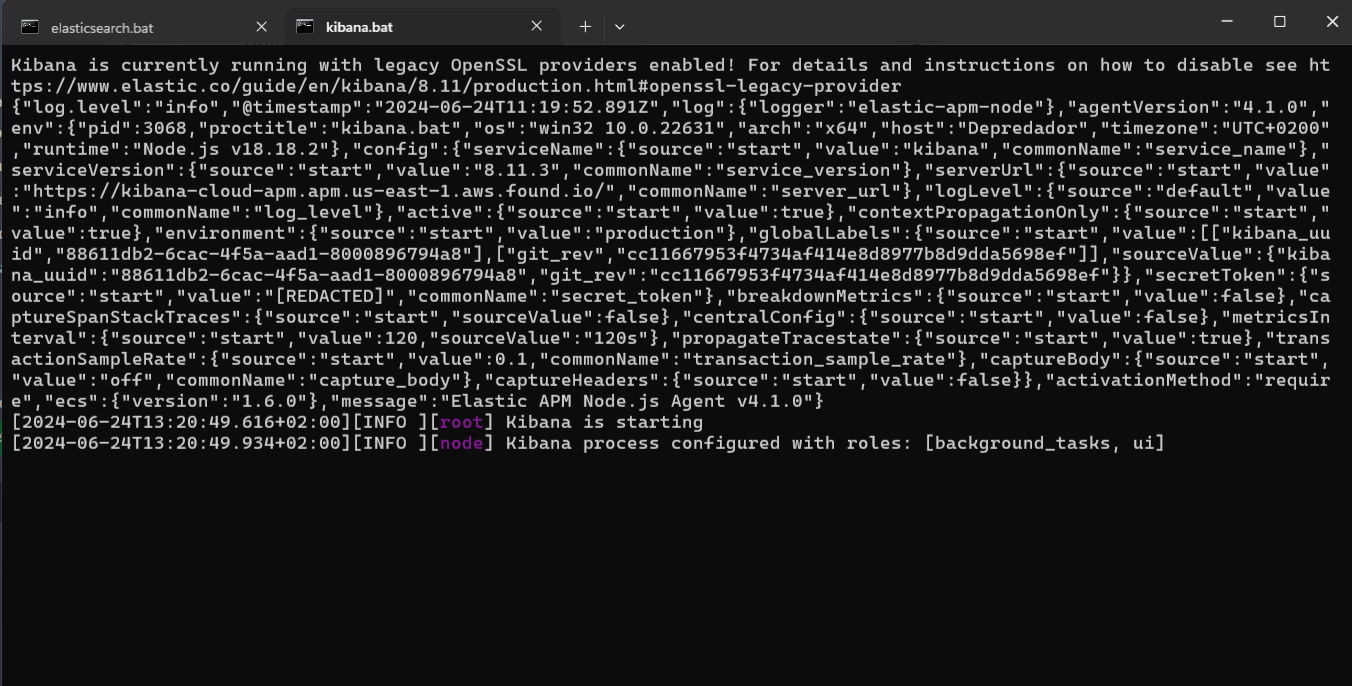
\includegraphics[width=1\linewidth]{img/kibanaa1.png}
    \caption{Visualización de terminal una vez se ejecute kibana.bat}
    \label{fig:kibana1}
\end{figure}

Pasados unos segundos, la terminal indicará que el servicio de Kibana está activo y para acceder a el nos iremos al navegador y nos dirigemos al puerto 5601, en el cuál se nos mostrará la interfaz gráfica de Kibana \ref{fig:kibana2}.

\begin{figure}
    \centering
    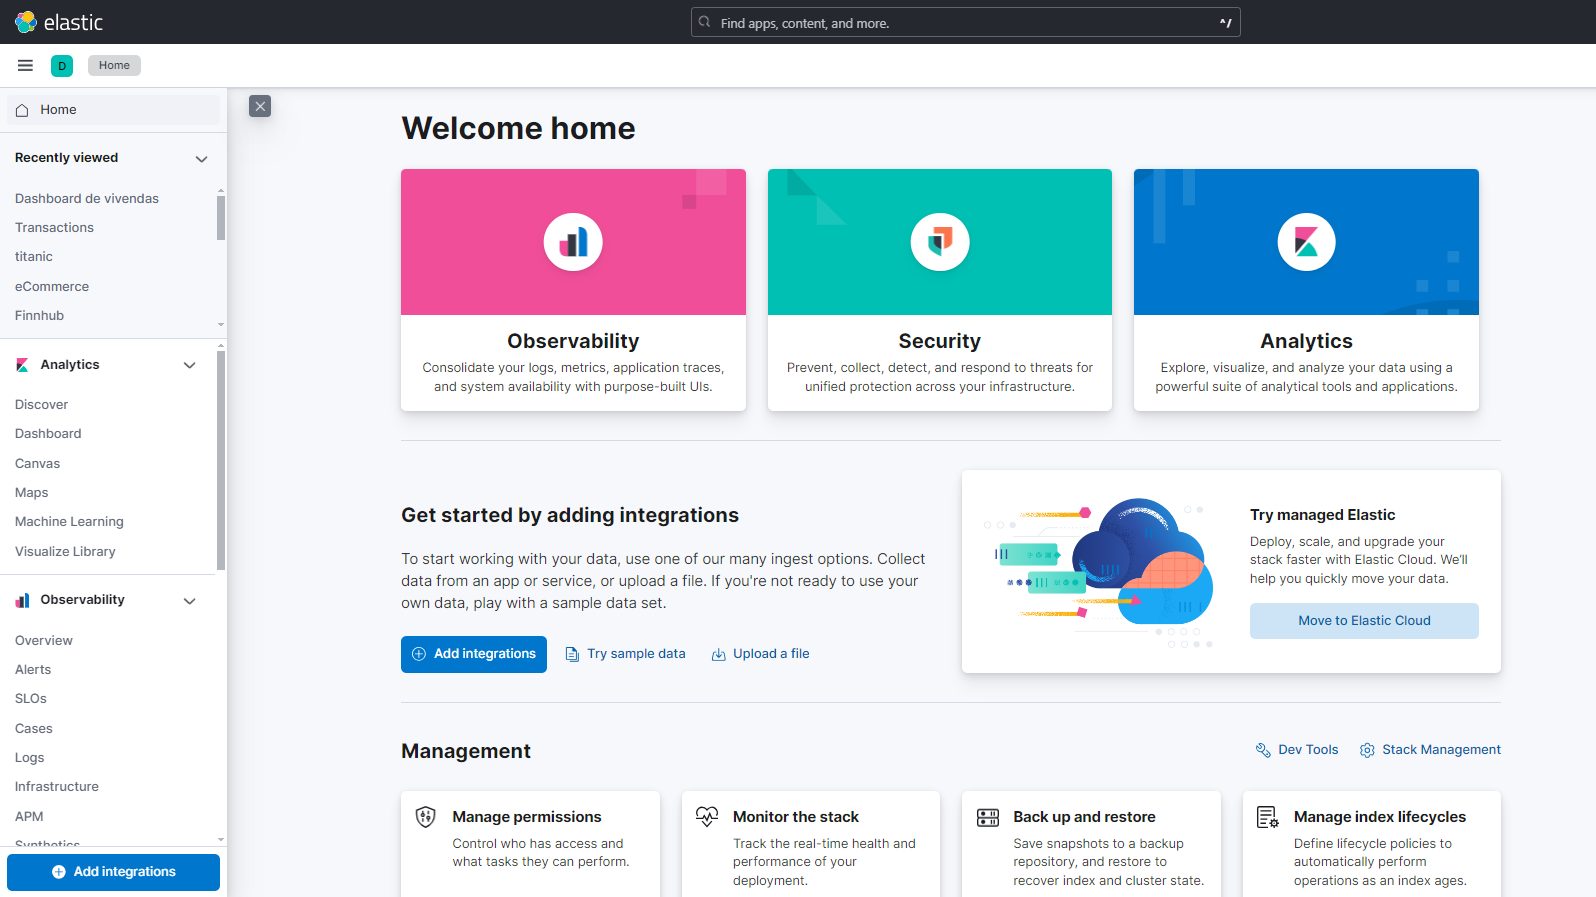
\includegraphics[width=1\linewidth]{img/kibana2.png}
    \caption{Interfaz gráfica inicial de Kibana.}
    \label{fig:kibana2}
\end{figure}

\paragraph{}
\paragraph{}
\paragraph{}
\paragraph{}


Una vez se llega a esta pantalla, se pueden observar las diferentes funcionalidades que ofrece Kibana. La primera en la que se va a indagar y que es importante de cara a comprobar que los datos de los índices de ElasticSearch son los deseados es la funcionalidad \textit{Analytics} \ref{fig:kibana3}. La parte que más interesa es la de \textit{Discover}, en la cuál se van a mostrar todos los registros presentes en el índice que se indique. En este ejemplo se van a visualizar los datos del índice \textit{titanic} \ref{fig:kibana4}, como se puede observar en la columna de la izquierda se muestran los campos disponibles junto al tipo al que pertenecen, pudiendo realizar filtrados personalizados pero no modificaciones. En la sección principal llamada \textit{Documents}, se muestran en detalle todos los datos de los registros presentes en el índice, permitiendo indagar más profundamente por si interesa alguno en concreto \ref{fig:kibana6}.

\begin{figure}
    \centering
    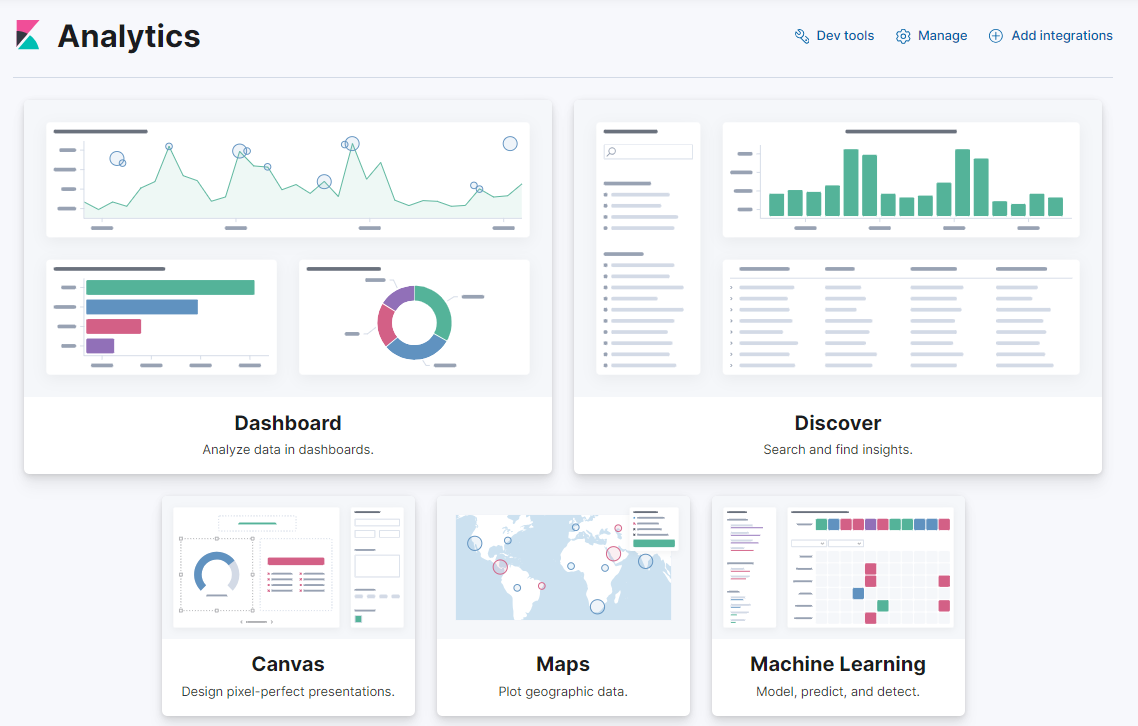
\includegraphics[width=1\linewidth]{img/kibana3.png}
    \caption{Visión general de la funcionalidad \textit{Analytics.}}
    \label{fig:kibana3}
\end{figure}

\begin{figure}
    \centering
    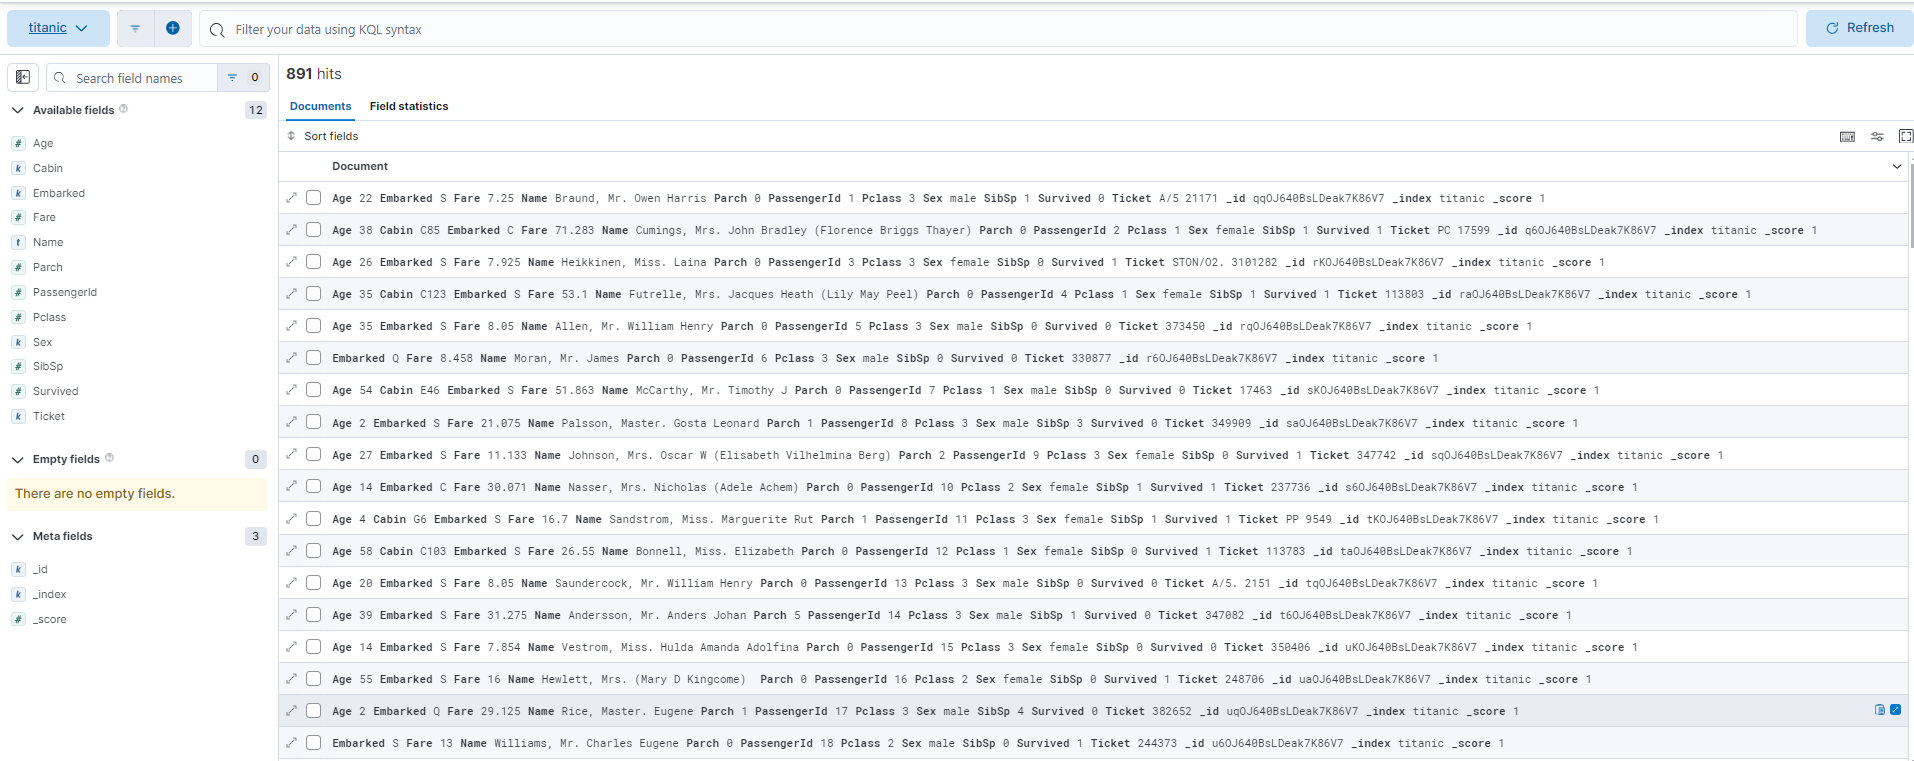
\includegraphics[width=1\linewidth]{img/kibana4.png}
    \caption{Visualización del \textit{Discover} de los datos del índice \textit{titanic}.}
    \label{fig:kibana4}
\end{figure}

\begin{figure}
    \centering
    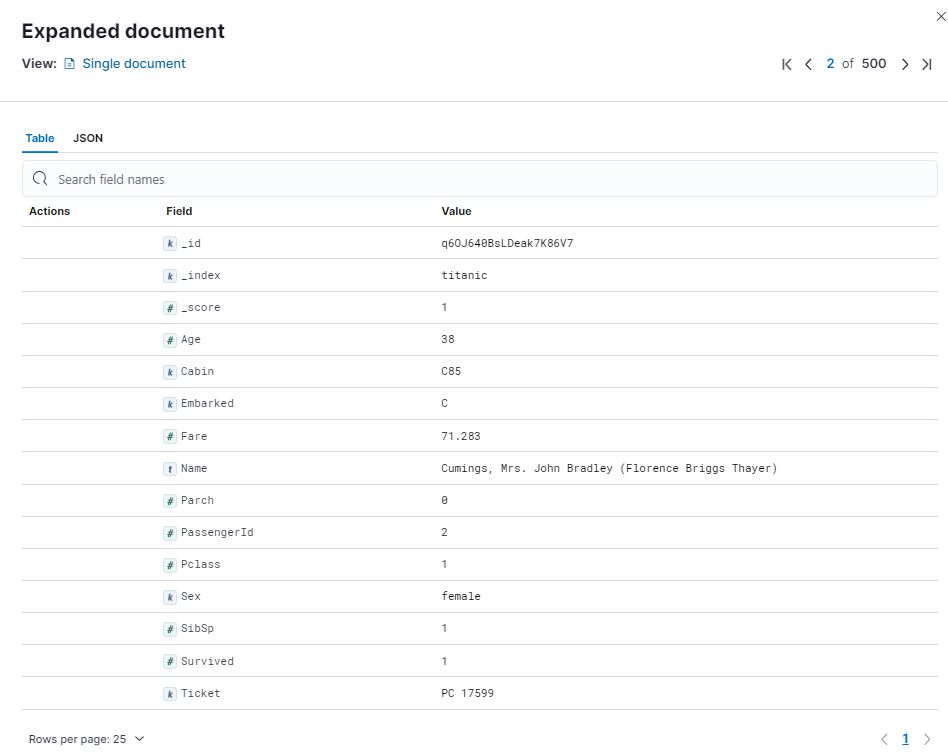
\includegraphics[width=1\linewidth]{img/kibana6.png}
    \caption{Visualización de un registro en concreto.}
    \label{fig:kibana6}
\end{figure}

Un apartado que resulta interesante de la funcionalidad \textit{Discover} es el de \textit{Field statistics} \ref{fig:kibana5}, en el cuál se muestran datos estadísticos útiles y precisos de cada campo presente en el índice, como pueden ser los valores únicos o la distribución de los valores.

\begin{figure}
    \centering
    \includegraphics[width=1\linewidth]{img/kibana7.png}
    \caption{Visualización de \textit{Field Statistics}.}
    \label{fig:kibana5}
\end{figure}

Una vez se tiene comprendido la funcionalidad \textit{Discover}, se puede pasar a la parte más interesante, que es la funcionalidad \textit{Dashboards} \ref{fig:kibana8}, en la cuál se realiza la parte más visual e intuitiva de todo el sistema ELK.

\begin{figure}
    \centering
    \includegraphics[width=1\linewidth]{img/kibana8.png}
    \caption{Visualización inicial de la funcionalidad \textit{Dashboards}.}
    \label{fig:kibana8}
\end{figure}

En esta sección, al igual que en la anterior, se va a indagar en el \textit{dashboard} proveniente del índice \textit{titanic}, equivalente al primero de los escenarios tratados.
La primera función a destacar es la de la posibilidad de filtrar los campos en función de los valores que se quieran \ref{fig:kibana9}. Los filtros se añaden desde la opción \textit{Controls}, pudiendo elegir si el filtro va a ser temporal o en función de los campos presentes. En este ejemplo se ha establecido un filtrado en función de la edad del pasajero \ref{fig:kibana10}, pudiendo configurar la etiqueta mostrada, el campo sobre el que se aplica el filtro o el tamaño que tendrá en el \textit{dashboard}.

\begin{figure}
    \centering
    \includegraphics[width=1\linewidth]{img/kibana9.png}
    \caption{Apartado de filtrado del \textit{dashboard}.}
    \label{fig:kibana9}
\end{figure}

\begin{figure}
    \centering
    \includegraphics[width=1\linewidth]{img/kibana10.png}
    \caption{Edición de un filtro del \textit{dashboard}.}
    \label{fig:kibana10}
\end{figure}

Antes de entrar en las visualizaciones, se quiere destacar la opción de permitir añadir un panel con toda la información de los datos sobre los que está trabajando el \textit{dashboard}, a modo de atajo sin entrar al \textit{Discover}. Esto se puede realizar desde la opción \textit{Add Library} \ref{fig:kibana11}, especificando el índice que se quiere mostrar.

\begin{figure}
    \centering
    \includegraphics[width=1\linewidth]{img/kibana11.png}
    \caption{Panel mostrando los datos del índice del \textit{dashboard}.}
    \label{fig:kibana11}
\end{figure}

\paragraph{}
\paragraph{}


Habiendo explicado estas funciones secundarias que ofrece la funcionalidad \textit{Dashboards} de Kibana, es momento de indagar en la función que permite crear visualizaciones con los datos del índice. Esto se realiza desde la opción \textit{Create visualization}. La visualización más sencilla es la de \textit{Metric}, en la cuál se puede especificar que se le aplique una función sencilla a un campo en concreto, en este ejemplo se ha hecho un conteo de todos los registros \ref{fig:kibana12}, y en este otro un conteo solo de los supervivientes con una fórmula usando sintaxis KQL \ref{fig:kibana13}.

\begin{figure}
    \centering
    \includegraphics[width=1\linewidth]{img/kibana12.png}
    \caption{Métrica del conteo del número de parajeros.}
    \label{fig:kibana12}
\end{figure}
\begin{figure}
    \centering
    \includegraphics[width=1\linewidth]{img/kibana13.png}
    \caption{Métrica de conteo del número de supervivientes.}
    \label{fig:kibana13}
\end{figure}

Otra visualización interesante es la de los gráficos de barras, en los cuáles hay que especificar que campo se quiere usar para cada eje, y si se quiere aplicar alguna función sobre los mismos.

En este ejemplo se está realizando un conteo del número de pasajeros clasificados por género \ref{fig:kibana14}, tomando como referencia el campo \textit{Género} para el eje horizontal representando en color azul los hombres y en rosa las mujeres, y el campo \textit{Records} para el eje vertical especificando que se realize un conteo de los valores.

\begin{figure}
    \centering
    \includegraphics[width=1\linewidth]{img/kibana14.png}
    \caption{Gráfico de barras mostrando el número de pasajeros por género.}
    \label{fig:kibana14}
\end{figure}

Otro tipo de visualización que resulta intersante es la del gráfico en forma de donut, en el cuál en este ejemplo se muestra el porcentaje de pasajeros por clase de billete \ref{fig:kibana15}, especificando que se va a realizar un filtrado por intervalos del campo \textit{Pclass} que es el que contiene la información pudiendo modificar las formas y colores del gráfico.

\begin{figure}
    \centering
    \includegraphics[width=1\linewidth]{img/kibana15.png}
    \caption{Gráfico de donut mostrando el porcentaje de pasajeros por clase de billete.}
    \label{fig:kibana15}
\end{figure}

Un gráfico presente en este \textit{dashboard} y que resulta interesante visualmente es el de un gráfico de barras apiladas, en este ejemplo se muestra en el eje horizontal la edad de los pasajeros y en el eje vertical el número de pasajeros estableciendo como diferencidador para el apilamiento el género de los mismos, esto se hace desde la función \textit{Breakdown} tomando como referencia los valores del campo \textit{Sex}.

\begin{figure}
    \centering
    \includegraphics[width=1\linewidth]{img/kibana16.png}
    \caption{Gráfico de barras apiladas mostrando la edad del número de pasajeros en función del género.}
    \label{fig:kibana16}
\end{figure}

Además de las visualizaciones mencionadas, Kibana ofrece visualizaciones similares en forma gráficos de barra horizontales, gráficos de area, mapas de calor o mosaicos. También incluye paneles más avanzados que requieren de datos más detallados como pueden ser mapas o streams de un log \ref{fig:kibana17}, en este \textit{dashboard} de la \href{https://www.elastic.co/es/blog/kibana-3-0-0-ga-now-available}{página oficial} de Kibana se pueden observar algunos de estos paneles \ref{fig:kibana18}.

\begin{figure}
    \centering
    \includegraphics[width=1\linewidth]{img/kibana17.png}
    \caption{Paneles más avanzados que ofrece Kibana.}
    \label{fig:kibana17}
\end{figure}

\begin{figure}
    \centering
    \includegraphics[width=1\linewidth]{img/kibana18.png}
    \caption{\textit{Dashboard} con paneles avanzados de Kibana.}
    \label{fig:kibana18}
\end{figure}

\paragraph{}
\paragraph{}


Una vez se da por finalizado la adición de visualizaciones y paneles al gráfico, este se puede guardar en el estado actual para poder ser modificado o exportado posteriormente desde la opción \textit{Save}. También se incluye una opción para visualizar el \textit{dashboard} como si se fuera un espectador desde \textit{Switch to view mode} \ref{fig:kibana19}, permitiéndo comprobar que todo está correcto.

\begin{figure}
    \centering
    \includegraphics[width=1\linewidth]{img/kibana19.png}
    \caption{Visualización general del \textit{dashboard} desde el modo espectador de Kibana.}
    \label{fig:kibana19}
\end{figure}

\apendice{Anexo de sostenibilización curricular}

\section{Introducción}
En los tiempos actuales, la sostenibilidad y el bueno uso de los recursos que se tienen son temas que han cobrado especial relevancia en todos los ámbitos de la vida. Por lo que en este anexo lo que se pretende es hacer una reflexión personal sobre como se han tratado estos temas a lo largo del estudio en los sistemas ELK.

\section{Impacto ambiental}
El impacto ambiental y social de las tecnologías que usamos en nuestro dia a dia cada vez es mayor, y una de las motivaciones de este TFG era comprender de que manera el uso de un sistema ELK puede ayudar a reducir el impacto ambiental de los sistemas de la información. Mediante la monitorización de procesos se reduce el uso de energía, ayudando a reducir el impacto en la huella de carbono, así como identificar ineficiencias operativas.

\section{Correcto uso de los recursos}
Para poder mejorar la sostenibilidad es clabe saber gestionar correctamente los recursos disponibles. En este estudio se han aplicado configuraciones para optimizar el rendimiento y reducir el consumo de estos recursos. Kibana permite identificar de manera más rápida y eficiente que áreas se pueden mejorar del proyecto así como ayudar a la toma de decisiones de cara a poder optimizar el uso de los recursos.

\section{Buenas prácticas}
Cabe destacar que a lo largo de este TFG se han hecho uso de prácticas responsables y éticas a la hora del manejos de los datos y la información, respetando tanto la privacidad como la seguridad de los datos procesados. Elastic a su vez permite usar medidas de seguridad para garantizar que solo los usuarios autorizados acceden y manejan la información sensible presente en el sistema.



\bibliographystyle{plain}
\bibliography{bibliografiaAnexos}

\end{document}
